\documentclass[
    twocolumn,
    fontsize = 10pt,
    parskip = half+,
    headings = small,
    headwidth = text,
    footwidth = text,
]{scrartcl}

\usepackage{pdflscape}
\usepackage{pgfgantt}
\usepackage{pdflscape}
\usetikzlibrary{shapes,backgrounds, arrows, positioning, trees, shadows}
\usepackage{pgf}
\usepackage{pgfplots}
\usepackage{pdflscape}
\usepackage{graphicx}
\usepackage{hyperref}
\pgfplotsset{compat=1.18}
\selectcolormodel{rgb}
\usepackage{booktabs}
\usepackage{array}
\usepackage{hyperref}
\usepackage{tabularx}
\usepackage{booktabs}
\usepackage{abstract}
\newcolumntype{Y}{>{\raggedright\arraybackslash}X}

\renewcommand{\arraystretch}{1.15}
\hypersetup{colorlinks=true,urlcolor=blue}

\KOMAoptions{
 paper = A4,
 pagesize,
 % headlines = 1.1,
 % headsepline,
 DIV = calc,
}
\typearea{11}

%\usepackage{fontspec}
%\setmainfont{Roboto Condensed}

\usepackage[
  todonotes={textsize=footnotesize},
  commandnameprefix=ifneeded,
  ulem={normalem,normalbf}
]{changes}
\definechangesauthor[name={Khalil Ben Larbi}, color=green]{kbl}

\usepackage{amsmath}

\usepackage[
  detect-all
]{siunitx}

\usepackage[
  style = ieee,
  backend = biber,
  hyperref = true,
  backref = true,
  seconds = true,
  date = iso,
]{biblatex}

\addbibresource{bib/bibliography.bib}

\usepackage{xurl}

\usepackage[acronyms=true]{glossaries}

\usepackage[
    colorlinks=true,
    allcolors=,
]{hyperref}

\usepackage[
    capitalize,
    nameinlink,
    noabbrev,
]{cleveref}

\newcommand{\rftvector}[1]{\underline{#1}}
\newcommand{\rftmatrix}[1]{\underline{\underline{#1}}}
\newcommand{\rftquaternion}[1]{\boldsymbol{#1}}

\newacronym{dfg}{DFG}{Deutsche Forschungsgemeinschaft}

\newacronym{rfi}{RFI}{Chair of Space Informatics and Satellite Systems}
\newacronym{rtg}{RTG}{radioisotope thermoelectric generator}

\newacronym{jmu}{JMU}{Julius-Maximilians-Universität Würzburg}

\newglossaryentry{cubesat}{
    name = CubeSat,
    description = {A small satellite following the form factor defined by the CubeSat Design Specification}
}

\makeglossaries

\title{Firmware for Gecko Testbed: Applications in Capturing Orbital Debris}
\author{
    \begin{minipage}[t]{.8\textwidth}
        \centering
         Ateeb Ahmed, Roshan Kumar Gupta, Vassilios Papadopoulos
    \end{minipage}
}
\date{August 20, 2025}

\begin{document}
\twocolumn[
\begin{@twocolumnfalse}

\maketitle

\begin{abstract}
Since the landmark space mission Apollo 11, there has been an exponential increase in man-made objects in space. Most of these objects orbit around Earth at varying altitudes and perform specific tasks like telecommunication, navigation (GPS), space-exploration and imaging (Hubble and James Webb Telescope) etc. Today there are 7,560 satellites orbiting Earth \cite{ucs}. These satellites are prone to failure due to extreme physical conditions and contribute to ever growing Space Debris. There are active efforts underway to capture such debris. To this end, this project explores suitability of Gecko Materials in applications of capturing and removing space debris. Specifically, we provide a firmware which enables researchers to control and program a testbed to evaluate and compare different types of gecko materials and their performance in space-like conditions. In the first section, we talk about the problem in more detail, describe the testbed and its components and finally lay out the requirements that needs to be satisfied by this software package. Second section breaks down the software package into its components and describes the working of each individual component in detail, further we also provide a step-by-step guide on how to use the developed User Interface, lastly this section also provides a table which lists all the requirements and contrast them against the developed features. Section 3, provides insights and discussion on the scope and findings of this project and future directions.


\end{abstract}
\end{@twocolumnfalse}
]


%------------------------------------------------------------------------------	
%------------------------------------------------------------------------------	
%------------------------------------------------------------------------------


\section{Introduction \textnormal{(By Ateeb  Ahmed)}}
In the last century mankind has made unprecedented technological advances and discoveries. Naturally, Space exploration, which has fascinated all civilizations that have existed, also had a breakthrough in the previous century when USA launched Apollo 11 on 26th July 1969 to Moon. While this project was mainly targeted to explore the lunar surface. Since then many other such objects are sent in space but only to perform specific tasks like communication, observation and scientific research. These objects usually orbit around Earth and are called Satellite. 
Currently, there are 7,560 satellites orbiting Earth \cite{ucs}. But keeping these satellites operational require constant maintenance since they are exposed to extreme temperatures, radiation and micro-meteoroids. Unfortunately, not all satellites stay operational through out their mission and gracefully leave the orbit. Some gets destroyed during deployment, or lose contact and control from Earth due to communication issues. These dead satellites and other small objects created due to some form of damage to existing satellites are collectively called "Space Debris". 
There are currently 32,750 cataloged and tracked debris objects, these 50 cm or more in size and traveling at a speed of 3 km/s \cite{space_junk}. \\

These objects also travel with a random trajectory and are not predictable. Collision with this debris can be fatal for not only existing operational satellites but also for future deployments. To this end, ClearSpace SA, a Swiss startup, is developing a device resembling a four-armed "space claw" that would grip junk satellites and de-orbit them. The project is expected to go live in late 2029, and intends to de-orbit a special kind of space debris called VESPA (Vega Secondary Payload Adapter) \cite{clear_space}. 

Recently, Gecko materials have shown promise in catching space debris [link]. Gecko materials exhibits certain properties which are desirable in space debris collection, such as: Gecko materials only require smooth surfaces. Gecko Materials do not require adhesive substance and work purely through fundamental property of materials called Van Der Waals forces. Due to these properties Gecko materials offer multiple docking opportunities to any space debris and offer good re-usability.

Given promising results from early proof of concept studies on Gecko materials for space debris collection, further research on how gecko materials behave in space-like conditions such as a combination of extreme temperatures, radiation, vaccume and microgravity is needed. 

In this regard, TU Berlin and Julius-Maximilian-Universität Würzburg as part of the \textbf{gEICko: GEcko based Innovative Capture Kit for uncooperative and unprepared Orbital assets} has initiated a joint investigation of Gecko materials. The team from TU Berlin has developed a Testbed. The goal of this Testbed is to compare different kinds of gecko materials against each other. The testbed is also suitable for simulated space-like environments since it is robust and vacuum sealed, a more detailed description of TestBed is provided in the following section.

This project, in particular, is concerned with developing a firmware to control the testbed and provide researchers with an intuitive but exhaustive user interface (UI) to be able to command and control this testbed.

\subsection{The Gecko Testbed}

\begin{figure}[h]
    \centering
    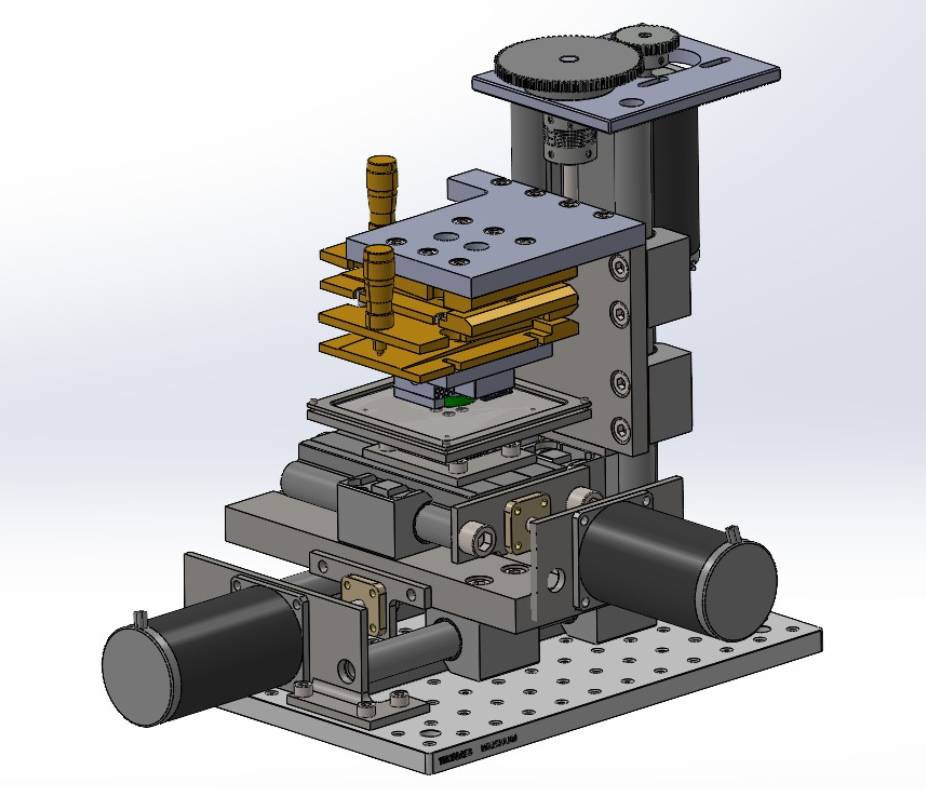
\includegraphics[width=1.0\linewidth]{pics/gecko_testbed.png}
    \caption{Testbed to test Gecko materials.}
    \label{fig: gecko testbed}
\end{figure}

Figure 1 shows an image of the testbed developed by the engineers from TU Berlin. This consists of 3 stepper motors. Each motor is responsible for movement in each direction i.e. x, y and z axes. In this center of the testbed is a smooth glass surface which simulates a smooth surface from that of a space debris and also serves as a rendezvous point aka point of contact. The small green piece directly on top of this surface represents the Gecko material being tested. The vertical motors (z-axis) moves the Gecko material up and down along its axis and press it against the smooth surface such that the gecko material stick to it.

There is also a small 3 dimensional force sensor right underneath the smooth surface which can sense press/pull forces as well as shear and translatory forces. 

The following are the exact specifications and details of each component of the Testbed:

\begin{itemize}
    \item Stepper Motor: 3 stepper motors are used in this testbed. Each stepper motor is controlled using CL57T driver.
    \item Force Sensor: We have used a Strain Guage Force Sensor by ME Systeme model K3D40 (10N). We have further used GSV-4USB amplifier to control force sensor and also to serialize the output.
    \item Power Supply: We have used a generic powersupply easily available in all labs at 24V and 1.5A.
    \item Computing Unit: We have used a Raspberry Pi micro-controller as our main computing device.
\end{itemize}

All of the components of the testbed mentioned above are shown in figure 2.

\begin{figure}[h]
    \centering
    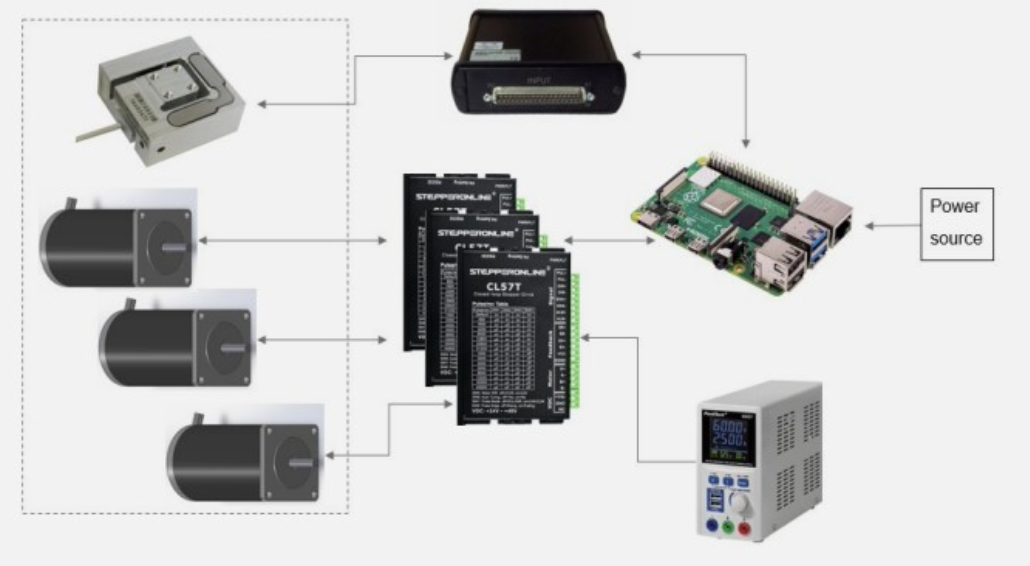
\includegraphics[width=1.0\linewidth]{pics/gecko_testbed_components.png}
    \caption{Individual Components of Gecko Testbed.}
    \label{fig: gecko testbed components}
\end{figure}


\subsubsection{Uses Cases of Testbed}
The main purpose for this testbed is to test and compare different gecko materials in space-like environments. The metric used to measure the effectiveness of a gecko material is the ratio between push and pull force generated, then an ideal Gecko material candidate would be one which requires minimum push forces against a smooth surface, sticks to it and then can pull the stuck surface with a much higher pull force.

This testbed accomplish this by pressing the gecko material against the smooth the surface until a target push force is reached (establishing docking), and then pull away the gecko material and measuring the pull force generated by gecko material. This simple experiment can have two further possibilities: 

\begin{itemize}
    \item Case 1: When smooth surface is static and only gecko material moves up and down.
    \item Case 2: When smooth surface is static until point of contact (docking), and while gecko material start pulling the smooth surface also moves along one or both horizontal axes (X and Y).
    \item Case 3: When the gecko materials establishes contact while smooth surface is moving along horizontal axes. Similarly, pull force is also measured with gecko and smooth surface moving. This case is the most complicated out of all above and accurately simulates the behavior of uncontrolled space debris.
\end{itemize}

Now that the use cases of the testbed are laid out, in the later sections we will describe how the developed firmware handles these situations. 



%------------------------------------------------------------------------------	
% Roshan's software sections begin here. Keep teammate sections below reserved.

\section{System Architecture \textnormal{(Delivered by Roshan Kumar Gupta)}}
\label{sec:system-architecture}

\subsection{Overview}
The developed testbed follows a three-layer architecture consisting of the frontend interface, the backend server, and the hardware integration layer. The goal of this design is to ensure modularity, real-time responsiveness, and safe interaction between user-defined sequences and the physical setup. Figure X illustrates the overall architecture of the system.

At the top layer, the web frontend acts as the primary interface between the user and the testbed. Implemented using Three.js and Vanilla JavaScript, the frontend provides a sequence builder for defining multi-axis actions, a real-time force graph, motor control buttons, and logging/export options. It communicates with the backend through REST API calls for commands and WebSocket events for live updates.

The backend server, built with Flask and Flask-Socket.IO, forms the middle layer of the system. It exposes endpoints for sequence execution, emergency stop, calibration, motor checks, and data export. Additionally, the backend streams force sensor readings, motor step counts, and experiment logs to the frontend in real time. This ensures the user has continuous visibility and control during experiments.

At the core logic level, the backend handles sequence execution, trigger evaluation (force, duration, step-based), and logging. Concurrency is achieved using threads, where a dedicated force poller thread continuously reads sensor data, while per-axis execution threads manage motor control. This modular approach allows the testbed to handle complex sequences while ensuring responsiveness to safety-critical events such as emergency stop signals.

The hardware interface layer provides low-level communication with the physical devices. GPIO control manages the stepper motors across three axes (X, Y, Z), while serial communication integrates the multi-axis force sensor. The Raspberry Pi 5 acts as the controller, bridging the backend software with the hardware. Feedback in the form of force measurements and step counts is continuously transmitted back to the backend and relayed to the user interface.

This layered architecture ensures a clean separation of concerns: the frontend focuses on visualization and usability, the backend manages logic and communication, and the hardware layer executes the actual physical tasks. Together, these modules form a reliable and extensible testbed for gecko adhesion experiments. 

\begin{figure}[htbp]
  \centering
  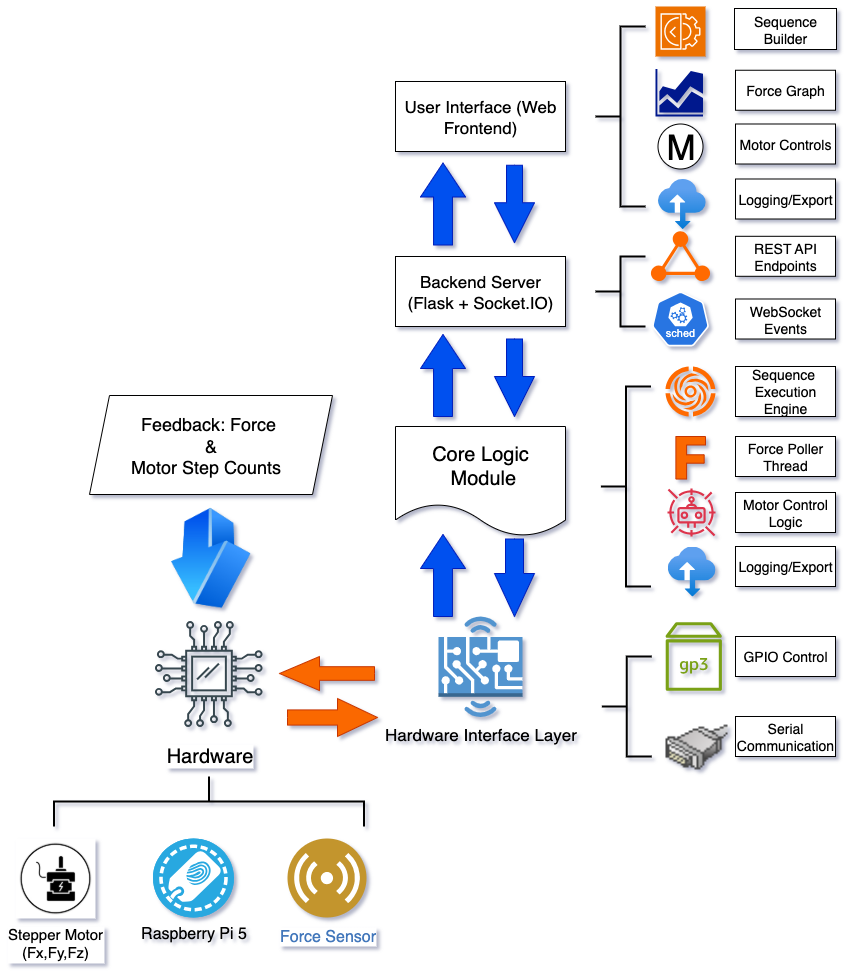
\includegraphics[width=\linewidth]{pics/gecko_architecture.drawio.png}
  \caption{Overall system architecture showing the web frontend, backend (Flask + Socket.IO), and hardware layer (Raspberry~Pi, motor drivers, force sensor) with data and control flows.}
  \label{fig:architecture}
\end{figure}


\subsection{Components}
\textbf{Frontend (Three.js + Vanilla JS):} Interactive StepBuilder, live telemetry ($F_x, F_y, F_z$, shear), per-axis step counts, 3D visualizer, and controls (Run, Stop, Emergency Stop (E-Stop), Motor Check, Zero Sensor, Repeat, Upload/Download State, Export Logs).\\
\textbf{Backend (Flask + Socket.IO):} HTTP actions for commands and JSON state, real-time event streaming, sequence execution threads, trigger evaluation, optional force-hold, logging, calibration/zeroing, and reset-to-origin.\\
\textbf{Hardware layer (Raspberry Pi + drivers + force sensor):} GPIO control for X/Y/Z stepper axes and a serial multi-axis force sensor. Feedback (forces, step counts) streams to the UI in real time.

\subsection{Data \& Control Flow}
(1) \emph{Authoring:} Define a sequence in the StepBuilder (movement, triggers, optional hold, Repeat) or upload a saved JSON.\\

(2) \emph{Dispatch:} The frontend sends a validated experiment description to the backend.\\

(3) \emph{Orchestration:} The backend runs a continuous force-poller thread and launches per-axis worker threads.\\

(4) \emph{Execution:} Workers step motors and evaluate triggers (``Any'' or ``All''). If a hold is configured, micro-movements maintain the target force until release conditions.\\

(5) \emph{Telemetry:} The backend emits \texttt{force}, \texttt{step\_count}, and \texttt{log} events; the UI renders them live.\\

(6) \emph{Lifecycle:} On completion—or Stop/E-Stop—the backend logs the outcome, resets axes to origin, and exposes a timestamped log for download. With Repeat, the full sequence executes $N$ times with clearly delimited iterations.

\subsection{Safety \& Fault Handling}
E-Stop immediately disables motion and raises a visible log event; a global force cap prevents out-of-range operation; Zero Sensor and calibration ensure stable force readings; reset-to-origin guarantees a known state between trials.

\subsection{Extensibility \& Constraints}
The modular design allows adding distance-based triggers, richer analytics, or a framework UI (e.g., Svelte/React) without changing core motion/telemetry logic. Real-time responsiveness depends on sensible step sizes, trigger thresholds, and hardware health.

% ------------------------------------------------------------------------------

\section{Frontend Implementation (Three.js + Vanilla JS) \textnormal{(Delivered by Roshan Kumar Gupta)}}
\label{sec:frontend}

\subsection{Role \& Goals}
The frontend is the \emph{operator console}: simple for non-technical users, responsive for live experiments, and strict enough to prevent unsafe setups. Priorities: clarity, low-latency feedback, guardrails, and repeatability/sharing of configurations.

\subsection{Three.js Scene}
(1) \emph{Scene graph:} world axes, camera (orbit controls), light rig, and minimal meshes to indicate stage/axes and motion direction.\\

(2) \emph{Rendering loop:} RequestAnimationFrame drives lightweight renders; UI updates are decoupled from the physics/control loops to keep 60 FPS when possible.\\

(3) \emph{Responsiveness:} layout adapts between wide desktop and narrow screens; critical controls remain above the fold.\\

(4) \emph{Safety affordances:} emergency stop is persistent and visually distinct; destructive actions require a single explicit click (no hidden combos).\\


\subsection{Interface Overview}
\textbf{Control Bar:} Run, Stop, E-Stop, Motor Check, Zero Sensor, Repeat (count), Upload/Download State, Export Logs.\\
\textbf{StepBuilder:} Per-axis steps with direction and step size; movement-init triggers; break triggers (force/duration/steps) with \emph{Any/All} logic; optional \emph{Hold} with release triggers.\\
\textbf{Telemetry Panel:} Live $F_x, F_y, F_z$ (and shear if shown) and per-axis step counts.\\
\textbf{3D Visualizer:} Three.js scene providing spatial context (axes, motion cues).\\
\textbf{Log Console:} Readable stream of step boundaries, trigger firings, hold state, stops, and errors.

\subsection{Interaction \& Workflows}
Configure or Upload a sequence; set Repeat for multi-trial tests; Run; monitor forces, step counts, logs, and 3D view; Stop (graceful) or E-Stop (immediate); Zero Sensor before force-critical runs; Motor Check for quick health; Download/Upload State to reuse setups; Export Logs for audit.

\subsection{Real-Time Behavior \& Safeguards}
WebSocket events are throttled to keep the UI responsive; forms validate unsafe combinations; connection status is visible; conflicting actions disable during active runs; E-Stop remains prominent.

% ------------------------------------------------------------------------------

\section{Backend Implementation (Flask + Socket.IO) \textnormal{(Delivered by Roshan Kumar Gupta)}}
\label{sec:backend}

\subsection{Role \& Boundaries}
The backend validates and executes sequences, manages concurrency and safety, streams telemetry, and persists an auditable log. It exposes clear actions: Run, Stop, E-Stop, Motor Check, Zero Sensor, Calibration, Repeat, State Upload/Download, and Log Export.

\subsection{Execution Model}
A dedicated force-poller thread continuously converts sensor frames to $F_x, F_y, F_z$ (plus $F_{\text{shear}}$) and broadcasts updates. Per-axis worker threads step motors and evaluate triggers concurrently. Serial I/O is lock-protected; shared state (forces, step counts) updates atomically. Long-running execution remains off the request thread so the API stays responsive.

\subsection{Trigger Engine \& Hold Control}
Triggers support force thresholds (with a global safety cap), duration, and step count; each group can require \emph{Any} or \emph{All}. Motion proceeds until break triggers are satisfied. When configured, a hold loop maintains a target force within tolerance until release conditions. Significant events (initiation, trigger fired, hold start/complete) are logged and streamed.

\subsection{Repeat \& Lifecycle}
A top-level Repeat count executes the full sequence $N$ times. Iterations are clearly delimited in the log. At run end (or stop), the backend resets axes to origin using tracked step counts, writes a timestamped log file, and clears transient state.

\subsection{Data, Logging \& State I/O}
During a run the backend buffers timestamps, force vectors, step counts, trigger events, step boundaries, and summaries; after a run it produces a uniquely named log file (Export Logs). Download State saves the current StepBuilder configuration as JSON; Upload State restores it for reproducible protocols.

\subsection{Robustness \& Safety}
Emergency Stop immediately drops motor control outputs and emits an operator log event; graceful stop halts at the next safe opportunity. The backend validates inputs and runs long-lived work off the request thread to keep the server responsive. A quick Motor Check routine verifies motion on each axis before full experiments; Zero Sensor and Calibration actions maintain a clean baseline and consistent units.

% ------------------------------------------------------------------------------

\section{Sensor Calibration \& Safety Mechanisms \textnormal{(Delivered by Ateeb Ahmed)}}
\label{sec:calibration}

\subsection{Calibration Method (Manufacturer Two-Point)}
Software scaling uses manufacturer-provided two-point calibration (0\,N, 10\,N). The default factors applied in software are listed in Table~\ref{tab:calibration-factors}. Raw frames are converted to physical forces per axis using these factors, and a \emph{Zero Sensor} action establishes a clean baseline before runs. Updated factors (from certificates or lab recalibration) can be applied and then re-zeroed.

\begin{table}[htbp]
\centering
\caption{Manufacturer-supplied two-point calibration factors (0\,N, 10\,N) used as software defaults.}
\label{tab:calibration-factors}
\begin{tabular}{|c|c|l|}
\hline
\textbf{Axis} & \textbf{Factor} & \textbf{Note} \\
\hline
$F_x$ & 0.0612932 & Provided by manufacturer \\
$F_y$ & 0.0603852 & Provided by manufacturer \\
$F_z$ & 0.052317133779699 & Provided by manufacturer \\
\hline
\end{tabular}
\end{table}


\subsection{Operator Workflow (Pre-Run)}
Zero Sensor with the fixture unloaded; verify factors; sanity-check idle $F_x, F_y, F_z$ are near zero; (optional) Motor Check; ensure StepBuilder thresholds respect the safety limit.

\subsection{Safety Envelope, Integrity \& Notes}
Global force cap (default 10\,N), ever-present E-Stop, graceful Stop, and post-run reset-to-origin ensure safe operation. The run log records timestamps, factors, zeroing actions, trigger events, step boundaries, and summaries; repeated runs are clearly delimited. Re-zero after fixture changes or temperature shifts; choose realistic setpoints.

% ------------------------------------------------------------------------------

\section{StepBuilder — Operator Guide \& Safety \textnormal{(Delivered by Ateeb Ahmed)}}
\label{sec:stepbuilder}

\subsection{Purpose}
``The StepBuilder is the control brain of the testbed (colloquially nicknamed `Thanos' during development for its make-or-break impact). It governs what to move, when to stop, and whether to hold a target force — per axis — for reproducible and safe experiments.''

\subsection{Core Concepts}
Step (per axis); movement-init triggers (preconditions); break triggers (force/duration/steps); optional Hold (maintain target force until release); \emph{Any/All} logic; experiment-level Repeat; State import/export; Log export.

\subsection{Recommended Workflow}
Define scope (Repeat or Upload a saved setup); configure steps (direction, step size; init/break triggers; optional Hold with release); validate (limits, Any/All logic, safe thresholds); run \& monitor (forces, steps, logs; Stop/E-Stop as needed); analyze \& reuse (Export Logs; Download State).

\subsection{Safety, Validation \& Recovery}
Keep thresholds within sensor range and below the safety cap; prefer force-based init triggers; E-Stop is always available; post-run reset to origin. Common mistakes: too many conditions with \emph{All}; unreachable holds; misunderstanding that Repeat applies to the \emph{entire} sequence; skipping Zero/Calibrate. Recovery: check init triggers/direction/step size; verify comparator and axis; re-zero for noisy holds; reconnect UI if needed.

% ------------------------------------------------------------------------------

\section{Operator Walkthrough: Using the Sequence Builder (Screenshots) \textnormal{(Delivered by Roshan Kumar Gupta)}}
\label{sec:sb-walkthrough}

This section shows, step by step, how a new operator or tester should use the \textbf{Sequence Builder} to configure and run experiments safely. Each step references a UI screenshot.

\paragraph{\textbf{Step 1 — Motor Check (unlock controls).}}
Open the UI and click \textbf{Motor Check} first. This verifies basic motion and unlocks run-time actions (Run/Stop/E-Stop).
\begin{figure}[htbp]\centering
  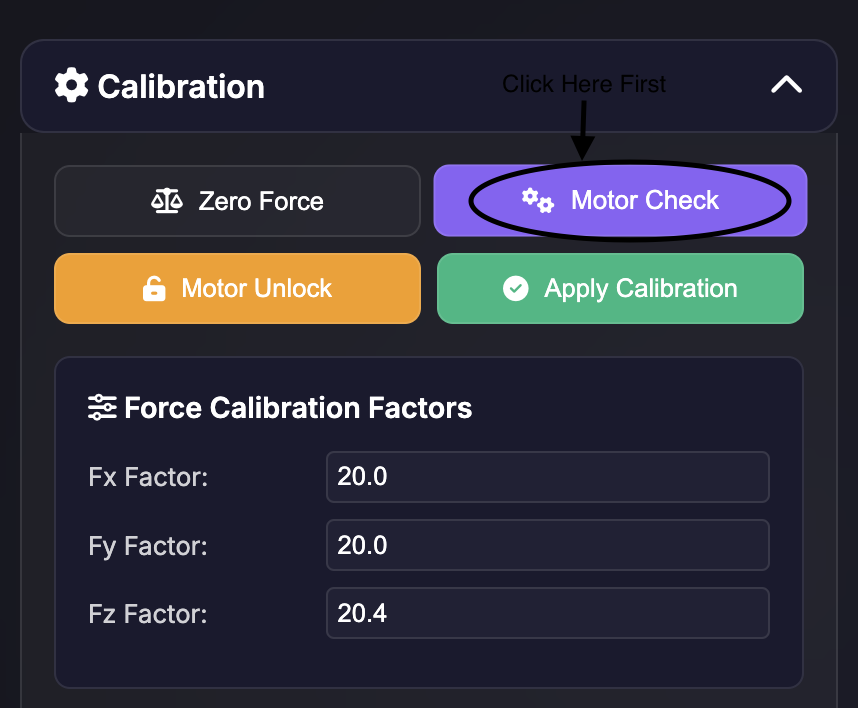
\includegraphics[width=.9\linewidth]{pics/motor-check.png}
  \caption{Run \textbf{Motor Check} to verify motion and unlock controls.}
  \label{fig:sb-motor-check}
\end{figure}

\paragraph{\textbf{Step 2 — Add a step (choose axis \& rate).}}
In \textbf{Sequence Builder}, click \textbf{Add X Step}, \textbf{Add Y Step}, or \textbf{Add Z Step}. Select direction and set the \textbf{Pulse Frequency (ms)} to control stepping rate.
\begin{figure}[htbp]\centering
  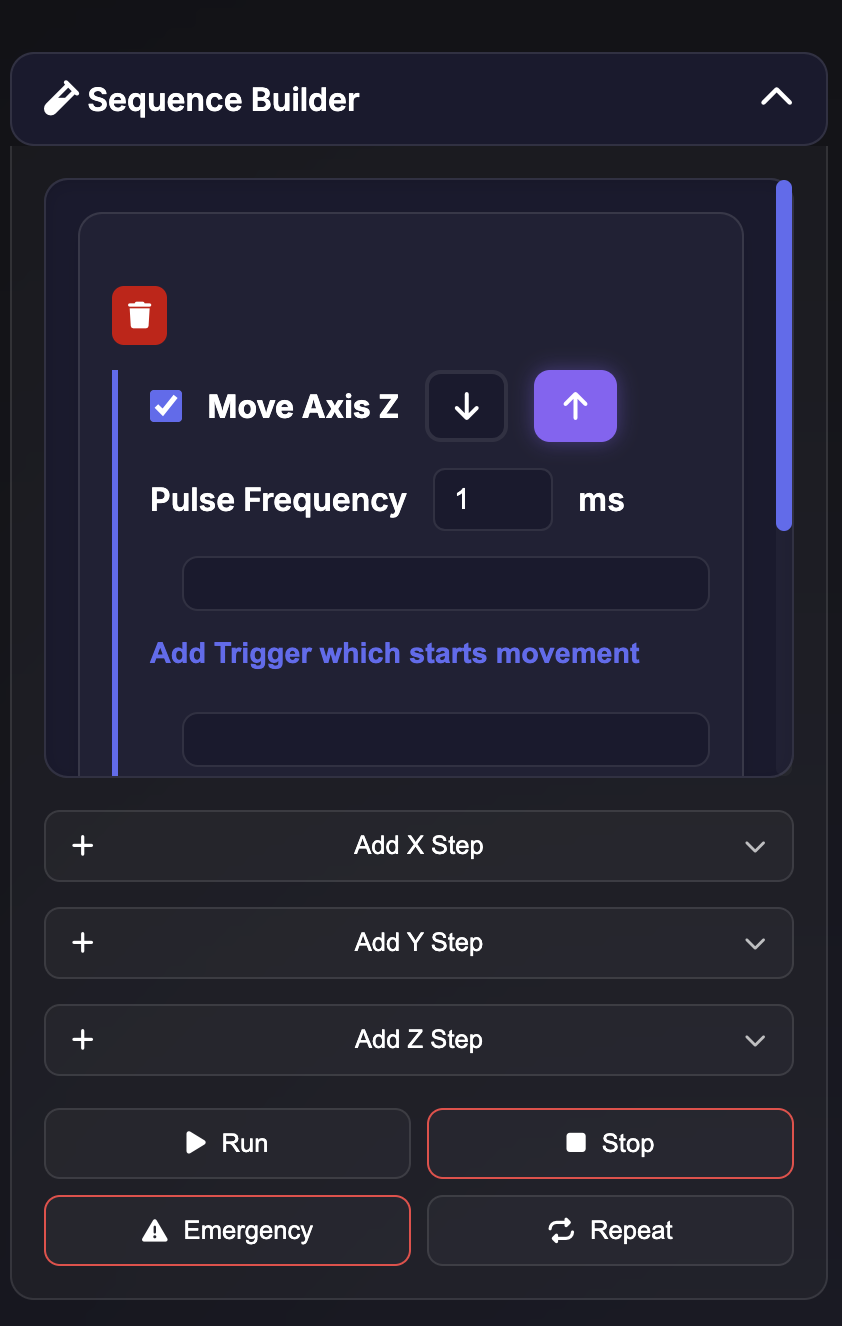
\includegraphics[width=.9\linewidth]{pics/sb-1.png}
  \caption{Add an axis step; set direction and \textbf{Pulse Frequency}.}
  \label{fig:sb-1}
\end{figure}

\paragraph{\textbf{Step 3 — Add a movement-init trigger.}}
Click \textbf{Add Trigger which starts movement}. Use this when the step must wait for a condition (typically a force threshold) before moving.
\begin{figure}[htbp]\centering
  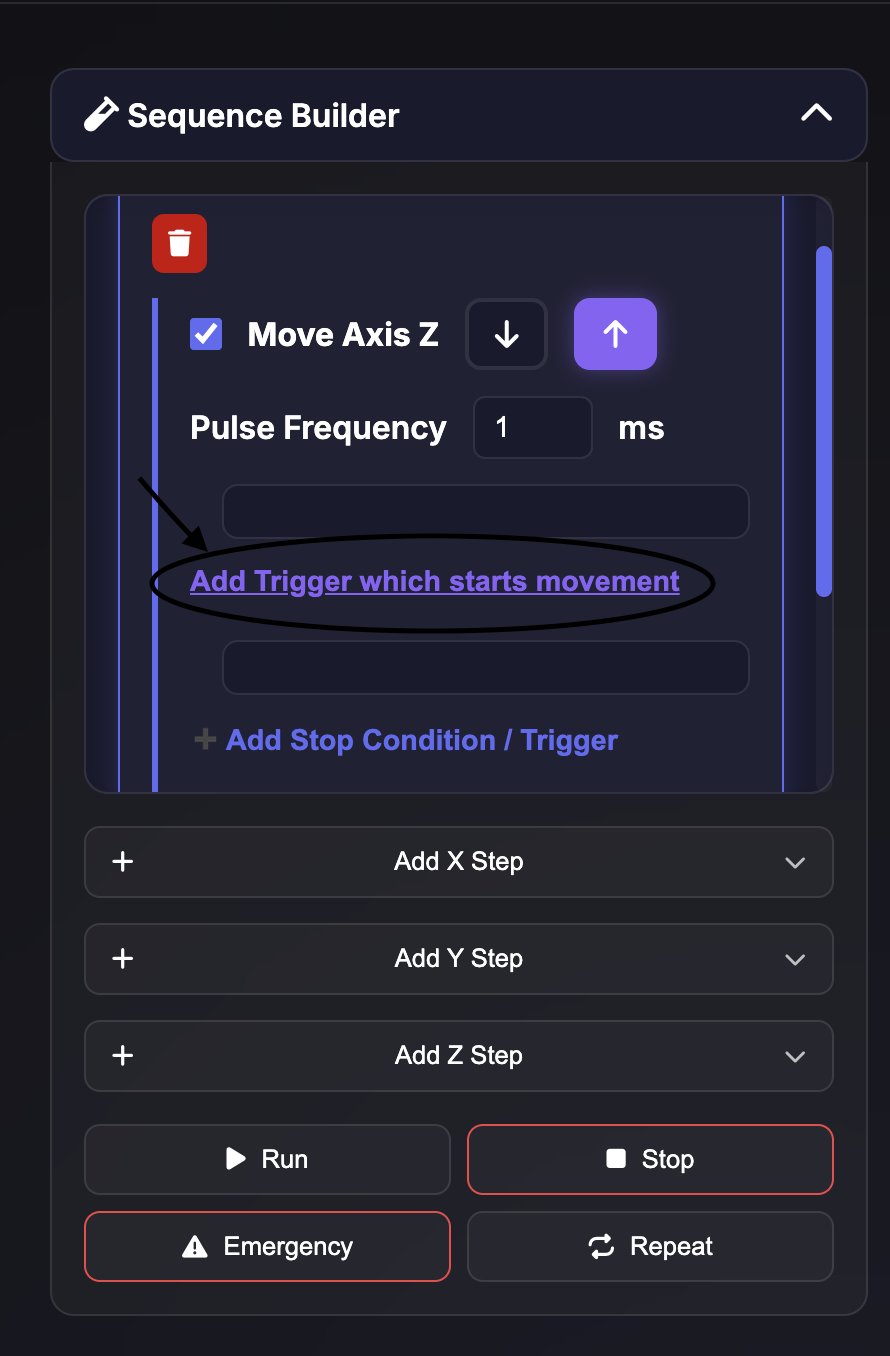
\includegraphics[width=.9\linewidth]{pics/sb-2.png}
  \caption{\textbf{Add Trigger which starts movement} to define preconditions before motion.}
  \label{fig:sb-2}
\end{figure}

\paragraph{\textbf{Step 4 — Configure the trigger.}}
Choose the signal (e.g., \textbf{Fz (N)}), comparator (\textbf{$\ge, \le, ==, >, <$}), and value (e.g., \textbf{1} = $1$\,N). \textbf{Fire All Triggers = True} requires all listed init triggers to be true; \textbf{False} means any one is enough. Checked axes move together; unchecked axes stay idle.
\begin{figure}[htbp]\centering
  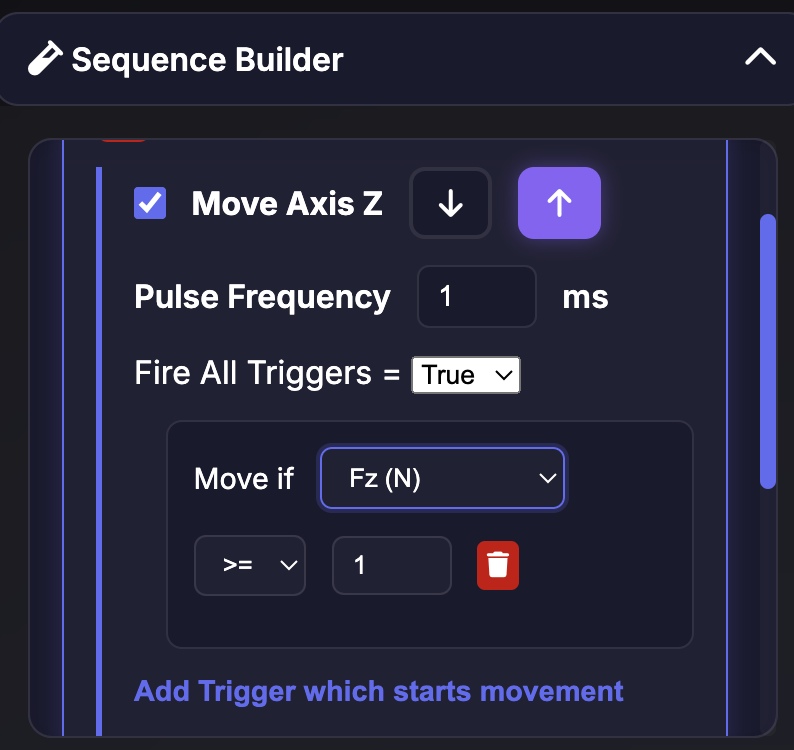
\includegraphics[width=.9\linewidth]{pics/sb-3.png}
  \caption{Configure a movement-init trigger: signal, comparator, and value.}
  \label{fig:sb-3}
\end{figure}

\paragraph{\textbf{Step 5 — Enable Hold Force.}}
Scroll to \textbf{Hold Force} and enable it to add a force-controlled hold after movement stops.
\begin{figure}[htbp]\centering
  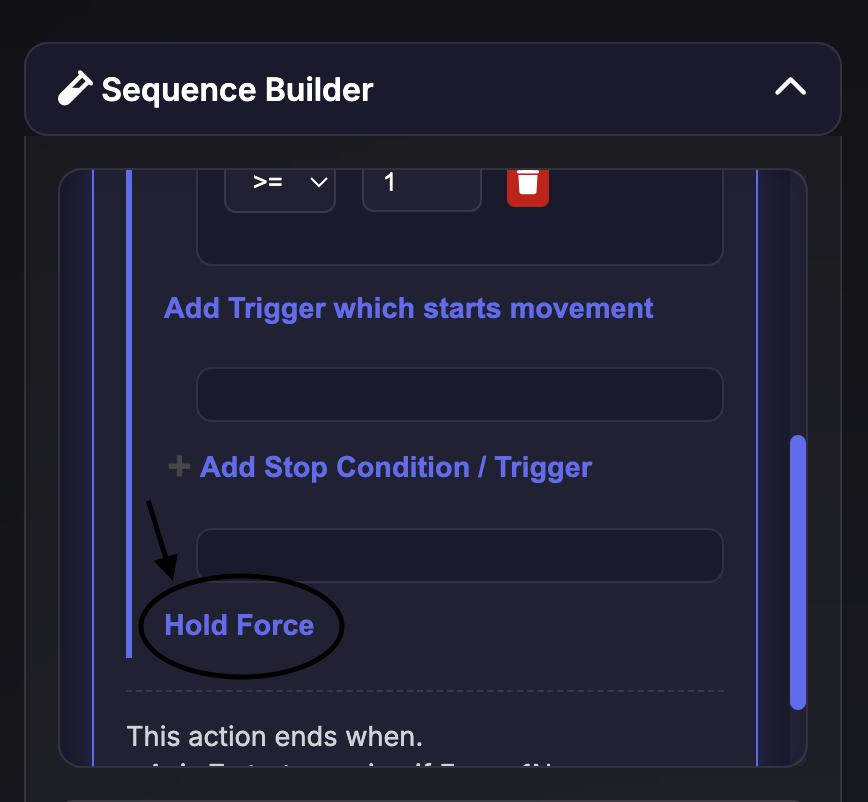
\includegraphics[width=.9\linewidth]{pics/sb-4.png}
  \caption{Enable \textbf{Hold Force} for a controlled force-maintenance phase.}
  \label{fig:sb-4}
\end{figure}

\paragraph{\textbf{Step 6 — Set Hold target and release conditions.}}
Enter the hold setpoint (e.g., \textbf{Hold Fz = 5\,N}) and add \textbf{Stop holding if} conditions (force/duration/step-count). 
\emph{Example:} If the break trigger is \textbf{Fz $\ge 10$\,N} and Hold is \textbf{5\,N}, the system presses until $\approx10$\,N, then settles and maintains $\approx5$\,N until the release condition fires.
\begin{figure}[htbp]\centering
  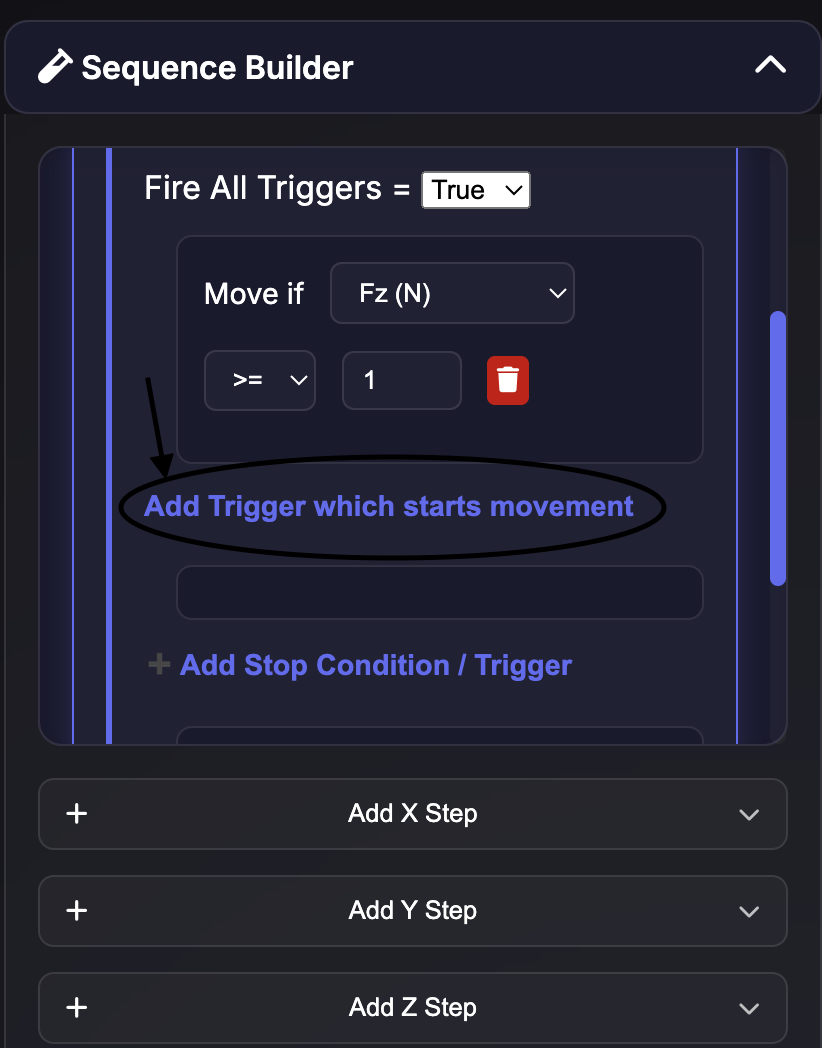
\includegraphics[width=.9\linewidth]{pics/sb-5.png}
  \caption{Set the \textbf{Hold} setpoint and release conditions.}
  \label{fig:sb-5}
\end{figure}

\paragraph{\textbf{Step 7 — Run once or enable Repeat.}}
Use \textbf{Run} to execute once, or enable \textbf{Repeat} to run multiple back-to-back trials for adhesion studies.
\begin{figure}[htbp]\centering
  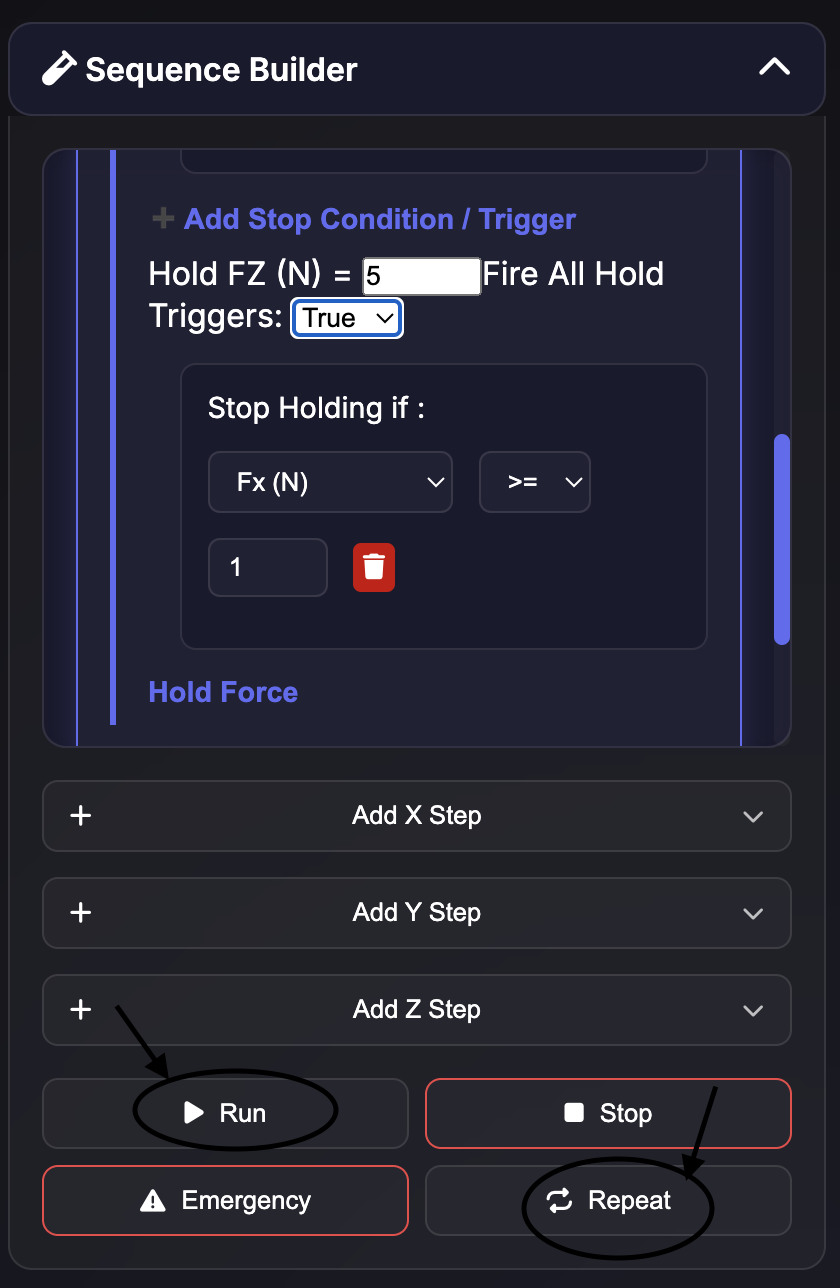
\includegraphics[width=.9\linewidth]{pics/sb-6.png}
  \caption{\textbf{Run} the sequence or enable \textbf{Repeat} for multiple trials.}
  \label{fig:sb-6}
\end{figure}

\paragraph{\textbf{Step 8 — Manage data (logs \& state).}}
\textbf{Export}: download the \textbf{timestamped} run log. 
\textbf{Upload}: load a saved \textbf{State (JSON)} to rehydrate the builder. 
\textbf{Download}: save the current builder state as JSON for reuse or sharing.
\begin{figure}[htbp]\centering
  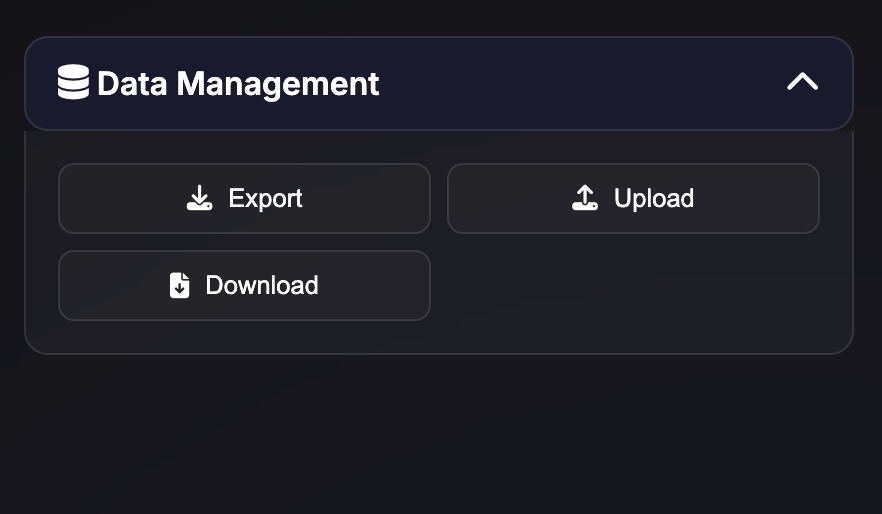
\includegraphics[width=.9\linewidth]{pics/sb-7.png}
  \caption{Data Management: \textbf{Export} logs; \textbf{Upload/Download State} JSON.}
  \label{fig:sb-7}
\end{figure}

\paragraph{\textbf{Step 9 — Monitor in real time \& use Manual Control.}}
Observe \textbf{X/Y/Z positions} and \textbf{Force (N)} during a run. The \textbf{Manual Control} panel uses \textbf{click-and-release} for safety—movement occurs only while the button is actively pressed (no continuous joystick).
\begin{figure}[htbp]\centering
  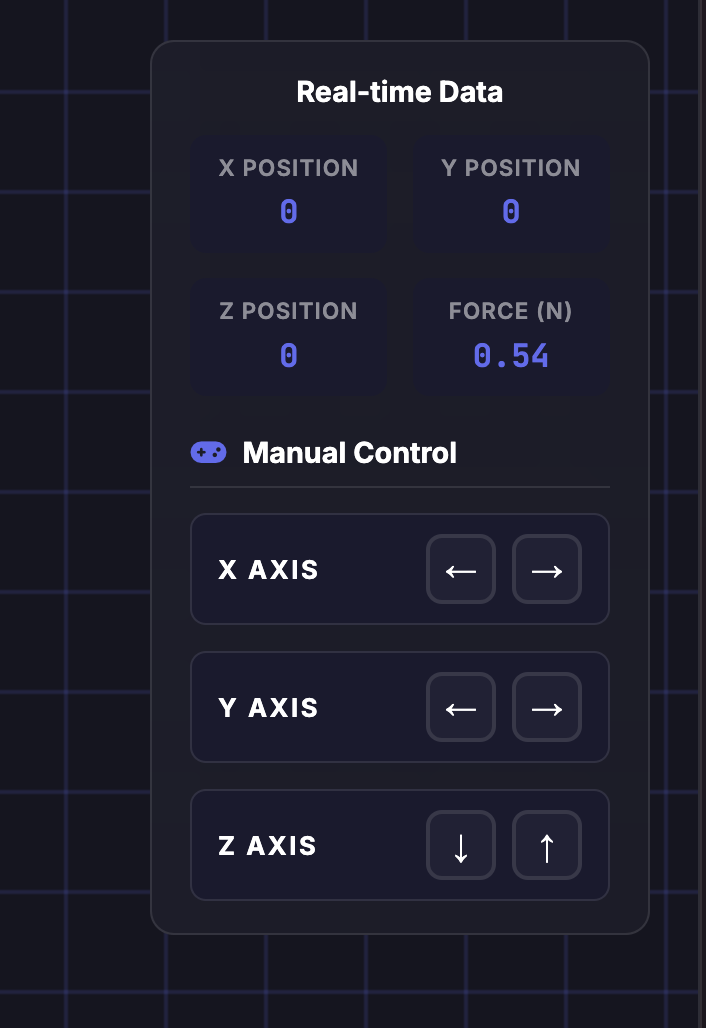
\includegraphics[width=.9\linewidth]{pics/sb-8.png}
  \caption{Real-time positions/force and \textbf{Manual Control} (click-and-release for safety).}
  \label{fig:sb-8}
\end{figure}


\paragraph{\textbf{Full UI overview (optional).}}
A wide view helps new users orient themselves: Sequence Builder (left), 3D scene (center), telemetry and logs (right/bottom).
\begin{figure}[htbp]\centering
  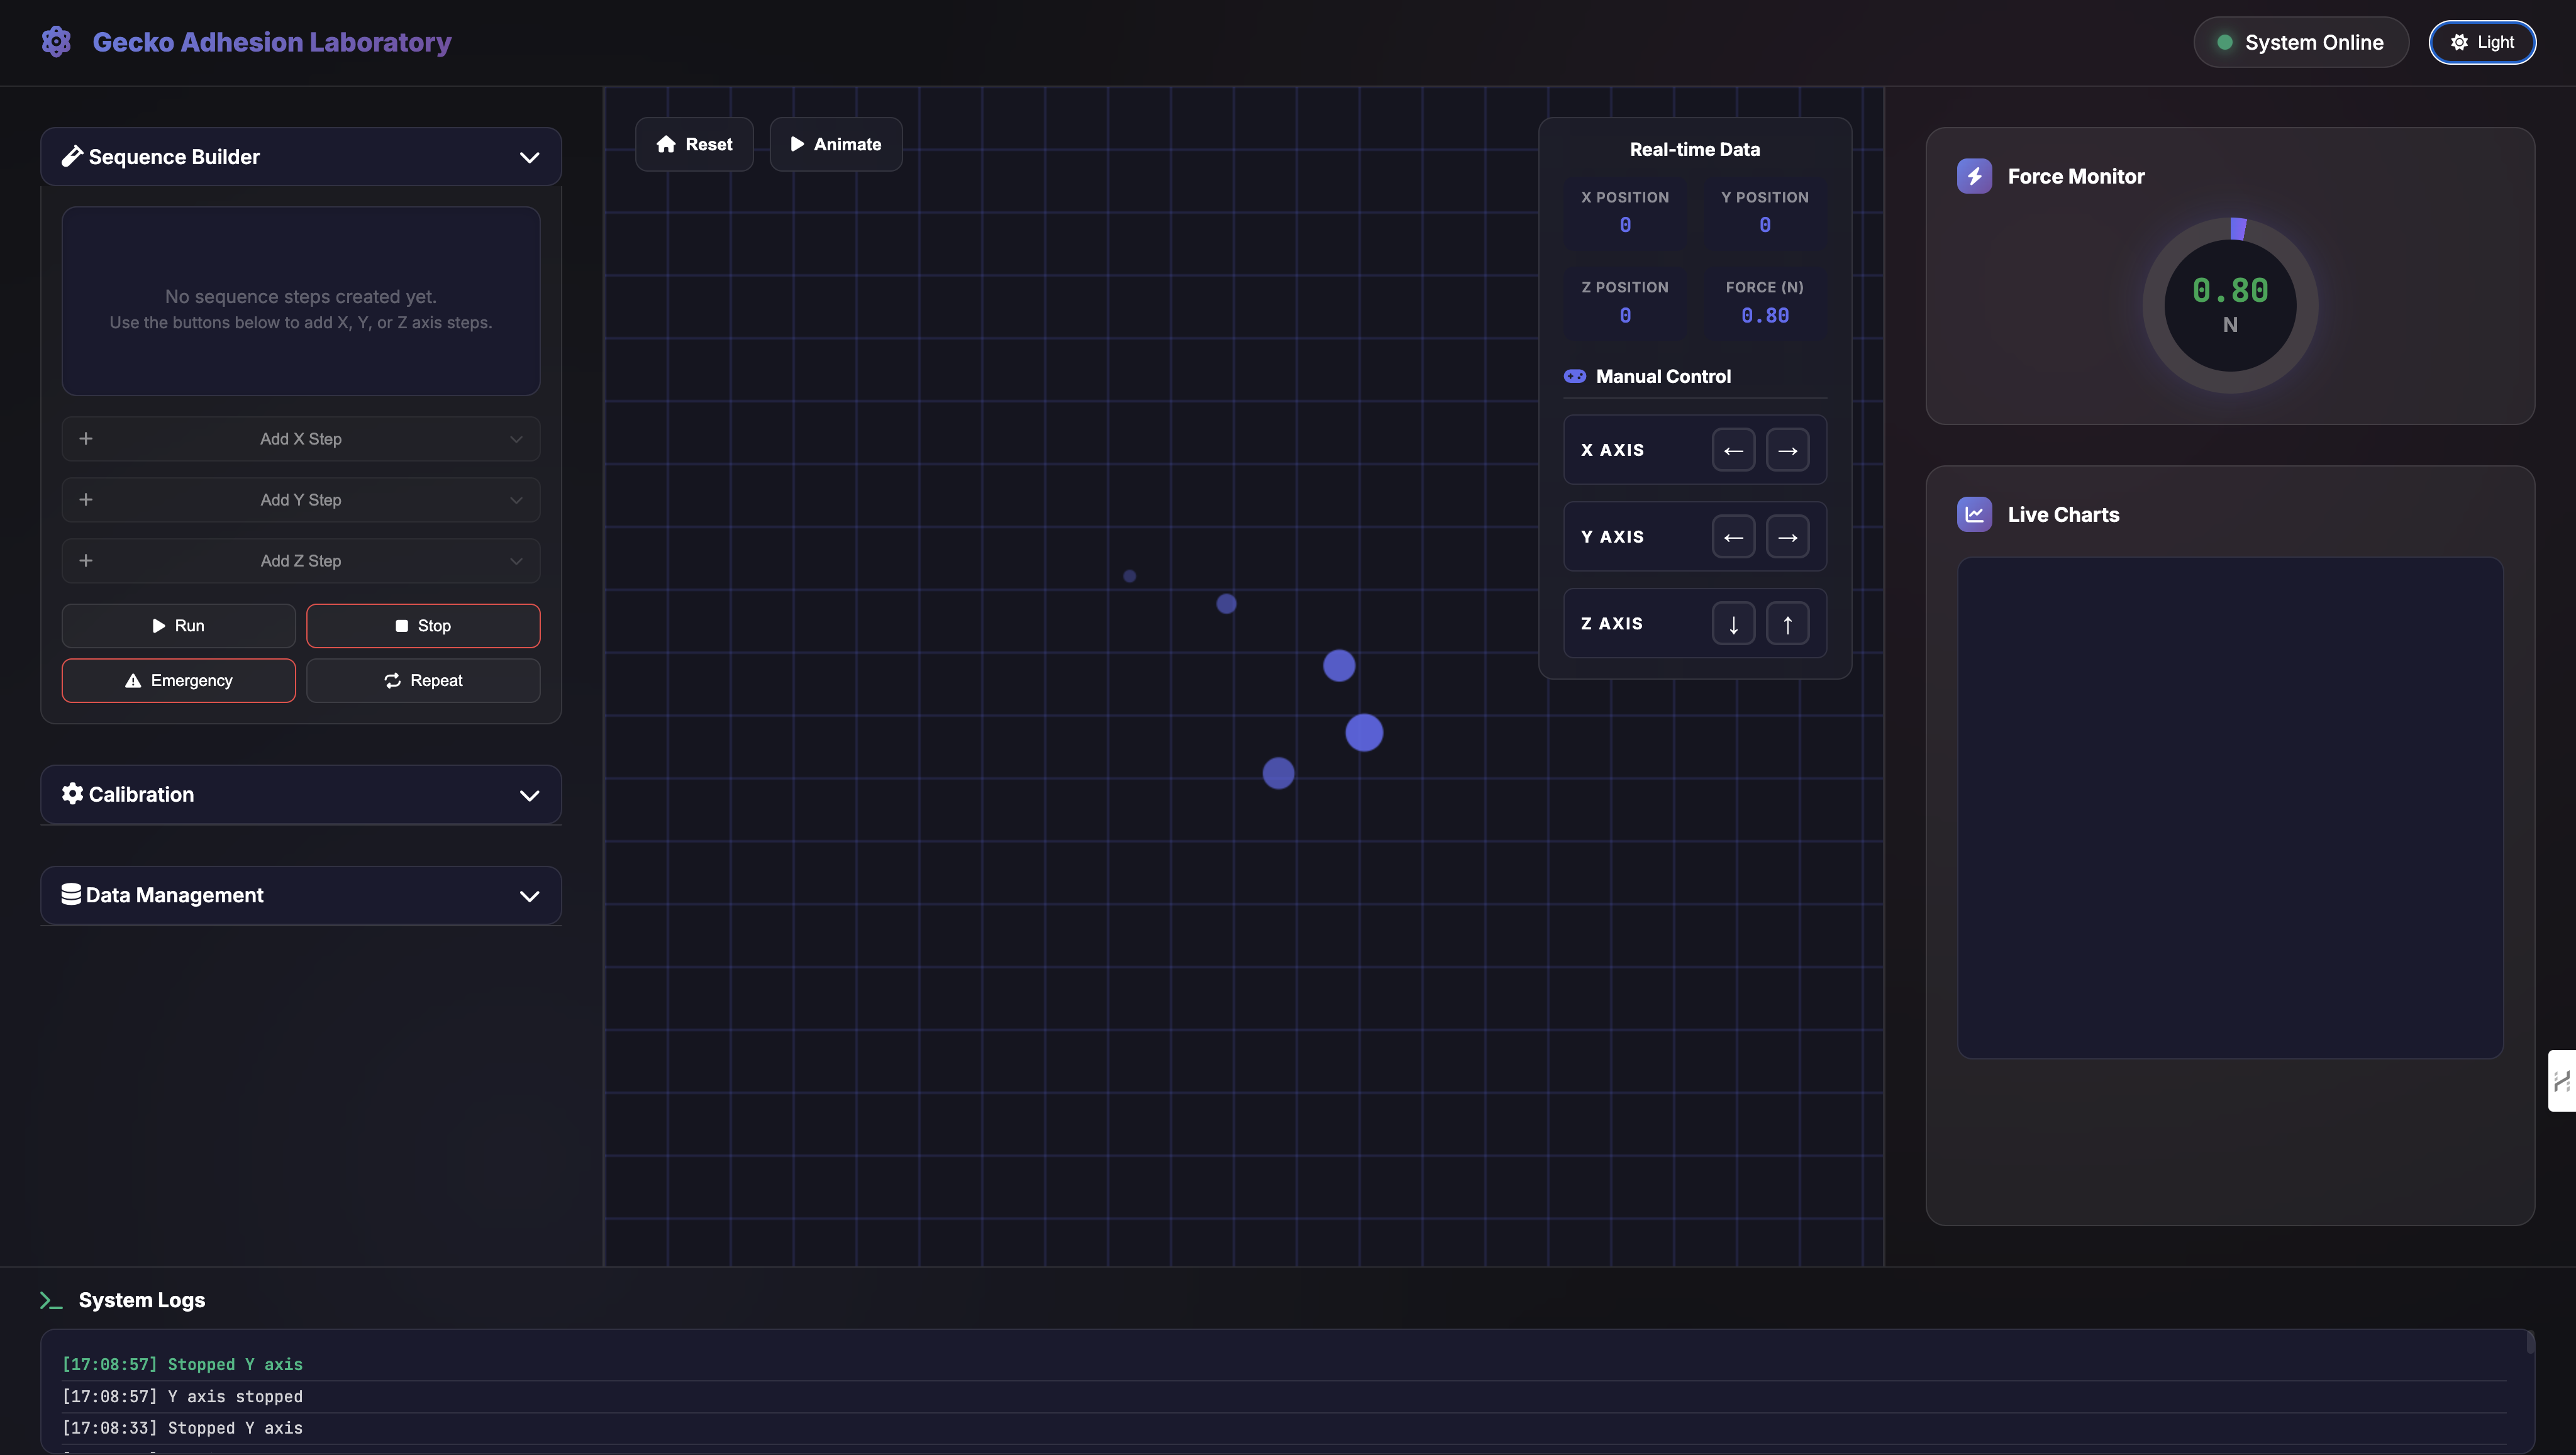
\includegraphics[width=\linewidth]{pics/ui-overview.png}
  \caption{Full UI overview of the Gecko Adhesion Laboratory dashboard.}
  \label{fig:ui-overview}
\end{figure}


% Where you want the link to appear(UI)
\noindent\href{https://roshangupta00750.github.io/geckotestbed/}
{\textbf{Get UI experience by clicking here}}
\textit{(some functionality won’t work as it’s not connected to the server).}\\
\textbf{Link:} \url{https://roshangupta00750.github.io/geckotestbed/}



\paragraph{\textbf{Notes \& tips.}}
\begin{itemize}
  \item Step-count triggers are available under \textbf{Add Stop Condition / Trigger} (e.g., stop after 2000 micro-steps).
  \item Keep thresholds within the sensor’s working range and below the global safety cap.
  \item \textbf{Emergency Stop (E-Stop)} is always available and halts motion immediately.
\end{itemize}


% ------------------------------------------------------------------------------

\section{Testing \& Results \textnormal{(Delivered by Roshan Kumar Gupta)}}
\label{sec:testing}

\subsection{Objectives}
Confirm safe, reproducible execution of user-defined sequences with real-time telemetry, Repeat trials, and post-run analysis via logs and state export.

\subsection{Test Plan}
(1) \emph{Functional:} Run/Stop/E-Stop, Motor Check, Zero/Calibrate, JSON Import/Export, Log Export.\\

(2) \emph{Execution:} Per-axis steps with movement-init, break, and optional hold.\\

(3) \emph{Repeatability:} Run the same sequence with Repeat to compare adhesion behavior.\\

(4) \emph{Telemetry:} Continuous $F_x, F_y, F_z$ (and shear where shown), step counts, and logs.\\

(5) \emph{Safety:} Force cap respected; E-Stop immediate; post-run reset to origin.

\subsection{Scenarios \& Expected Outcomes}
Approach-until-contact (``$F_z \ge$ threshold'') halts at the threshold with a trigger-fired log; 
force-controlled hold maintains setpoint until release; 
Repeat produces delimited iterations with reset between runs; 
mid-motion E-Stop halts immediately and logs the event; 
state I/O round-trip rehydrates and exports as expected.

\subsection{Evidence (Artifacts)}
Screenshots: dashboard during run; Repeat setting + per-iteration headers; excerpt of exported log (step starts/stops, triggers, holds); Upload/Download State flow confirming round-trip.

% ---------- 8.4 Evidence (Artifacts) — Part A ----------
\begin{table*}[t]
\centering
\caption{Requirement $\rightarrow$ Evidence Traceability (Section 8.4)}
\label{tab:traceability-a}
\setlength{\tabcolsep}{4pt}
\renewcommand{\arraystretch}{1.15}
\footnotesize
\begin{tabularx}{\textwidth}{@{}p{.24\textwidth}YYY@{}}
\toprule
\textbf{Requirement (what)} & \textbf{Implementation (where)} & \textbf{Report Section} & \textbf{Evidence (figure/file)} \\
\midrule
End-to-end run of a user-defined sequence
& Backend per-axis worker threads execute steps; StepBuilder defines steps/triggers
& §§ 3, 4, 6–7
& Fig.~\ref{fig:sb-6} “Run/Repeat”; \texttt{LOG-1} exported run log \\
Movement-init triggers supported
& Trigger evaluation before stepping (force preconditions)
& §§ 4.3, 6.2, 7 (Steps 3–4)
& Fig.~\ref{fig:sb-2} “Add Trigger which starts movement”; Fig.~\ref{fig:sb-3} configured trigger \\
Break triggers: \textbf{force / duration / steps}
& Trigger engine with comparators ($\ge, \le, ==, >, <$)
& §§ 4.3, 6.2, 7 (Steps 5–6)
& Fig.~\ref{fig:sb-4} “Add Stop Condition / Trigger”; Fig.~\ref{fig:sb-5} release conditions \\
Optional \textbf{Hold} (maintain target force) with release conditions
& Hold control loop with corrective micro-moves
& §§ 4.3, 6.2, 7
& Fig.~\ref{fig:sb-4} enable Hold; Fig.~\ref{fig:sb-5} Hold $=5$\,N + release \\
\textbf{Any/All} trigger logic
& Config flag for trigger groups
& § 6.3; 7 (Step 4)
& Fig.~\ref{fig:sb-3} “Fire All Triggers = True” \\
\textbf{Repeat} full experiment $N$ times
& Repeat lifecycle wraps entire sequence; iterations logged
& § 4.4; 7 (Step 7)
& Fig.~\ref{fig:sb-6} “Repeat = N”; \texttt{LOG-1} shows “Execution 0/1/…” \\
\textbf{Emergency Stop} immediate halt
& E-Stop drops outputs and broadcasts event
& §§ 3.4, 4.6, 6.4
& Fig.~\ref{fig:sb-6} “Emergency” button; \texttt{LOG-1}: “Emergency stop: All motors halted.” \\
\textbf{Graceful Stop}
& Stop at the next safe point
& §§ 3.4, 4.6
& Fig.~\ref{fig:sb-6} “Stop”; \texttt{LOG-1}: “Stopping …” then reset \\
\textbf{Motor Check} health routine
& Backend quick forward/back per axis + logs
& §§ 3.3, 4.6
& Fig.~\ref{fig:sb-motor-check} motor check \\
\textbf{Zero Force} baseline \& \textbf{Calibration} factors
& Zeroing + Apply Calibration in UI; software scaling
& §§ 3.3, 5.1–5.2
& Fig.~\ref{fig:sb-motor-check} “Zero Force” / “Apply Calibration”; Table~\ref{tab:calibration-factors} \\
\textbf{Global force safety cap} respected
& Safety bound in trigger evaluation
& §§ 5.3, 6.4
& \texttt{LOG-1}: no overshoot beyond cap during runs \\
Live \textbf{Fx/Fy/Fz} (and shear) telemetry
& Socket.IO streams; UI telemetry panel
& §§ 3.4, 4.2
& Fig.~\ref{fig:sb-8} real-time panel; Fig.~\ref{fig:ui-overview} \\
Live \textbf{step counts} per axis
& Backend emits counts; UI status
& §§ 3.4, 4.2
& Fig.~\ref{fig:sb-8} \\
\textbf{3D visualizer} (spatial context)
& Three.js scene with axes/motion cues
& § 3.2
& Fig.~\ref{fig:ui-overview} full UI \\
\textbf{State Export/Import (JSON)}
& Download current setup; Upload to rehydrate
& §§ 3.3, 4.5, 7 (Step 8)
& Fig.~\ref{fig:sb-7} “Export / Upload / Download”; \texttt{STATE-1} JSON file \\
\textbf{Log export} for analysis
& Timestamped human-readable log file
& §§ 3.3, 4.5, 9
& \texttt{LOG-1} exported file (attach) \\
\textbf{Post-run reset to origin}
& Walk-back using tracked steps
& §§ 4.4, 6.4, 9
& \texttt{LOG-1}: “Resetting motors to initial state.” \\
\textbf{Manual Control} safety mode
& Click-and-release (no continuous joystick)
& §§ 3.2, 7 (Step 9)
& Fig.~\ref{fig:sb-8} manual controls \\
\textbf{Interactive UI preview (web)}
& Static demo of the interface
& Artifacts / Appendix
& \href{https://roshangupta00750.github.io/geckotestbed/}{Get UI experience here} — \url{https://roshangupta00750.github.io/geckotestbed/} \\
\bottomrule
\end{tabularx}
\end{table*}


\section{Conclusion \textnormal{(Delivered by Vassilios Papadopoulos)}}

\subsection{Validation of the Testbed on Earth}

The developed gecko-inspired adhesion testbed has first been validated under terrestrial laboratory conditions. 
Initial experiments demonstrated that the combination of a high-precision force sensor and automated software control loops 
allows for reproducible adhesion and detachment measurements across a large number of cycles. 
Unlike manual test procedures, which are limited by operator accuracy and fatigue, the automated system can execute 
precisely defined loading–unloading sequences with high repeatability. 
This capability is critical for assessing long-term performance of micropatterned dry adhesives (MDA), 
where subtle changes in force profiles over hundreds or thousands of repetitions may indicate degradation of surface structures or material fatigue.  

The integration of software-based closed-loop control further enhances the stability of the experimental setup. 
The implemented routines manage motor speed, preload forces, dwell times, and detachment trajectories in a way that minimizes variability between test runs. 
This not only improves confidence in the measurement data, but also reduces human-induced bias. 
Particularly for adhesives whose performance depends strongly on contact geometry and loading history, 
automation is indispensable to generate meaningful datasets for later comparison with results obtained in microgravity environments.  

A key feature of the testbed is its ability to maintain constant normal forces during adhesion testing. 
Force feedback from the sensor is processed in real time by the control software, 
enabling rapid adjustment of the actuator position to compensate for surface irregularities or environmental disturbances. 
This ensures that the desired preload values are applied consistently, a prerequisite for studying the sensitivity of gecko adhesives to initial contact conditions.  

Moreover, the validation phase confirmed the robustness of the hardware components. 
The linear actuator, load cell, and mounting frame remained stable under extended operation, 
allowing tests of several thousand adhesion cycles without measurable drift in calibration. 
This establishes the platform as a reliable tool for systematic material studies, paving the way for subsequent adaptation to reduced-gravity scenarios.  

In summary, the terrestrial validation confirms that the testbed provides accurate, repeatable, and scalable measurement of gecko-inspired adhesives. 
This baseline is essential before transferring the system to constrained environments such as parabolic flights, drop tower experiments, or even orbital missions.


\subsection{Scalability to Microgravity Platforms}

While the testbed has proven effective under terrestrial conditions, 
its true potential lies in adapting the hardware and software for operation in reduced-gravity environments. 
Several experimental platforms are available within Europe that provide access to microgravity conditions, 
each with unique constraints in terms of duration, size, power availability, and environmental robustness. 
The following subsections outline how the testbed can be scaled and adjusted to these platforms, 
highlighting both the opportunities and limitations of each environment.

\subsubsection{ESA Fly Your Thesis}
Parabolic flights provide repeated intervals of approximately 20~seconds of microgravity per parabola. 
This offers the advantage of a relatively high number of test repetitions within a single campaign, 
allowing different adhesive samples or loading regimes to be investigated under similar flight conditions. 
However, the short duration of each microgravity phase requires highly efficient and fast experimental routines, 
forcing a trade-off between motor speed and precision of the applied motion profiles.

To meet the constraints of parabolic flight, significant modifications to the current testbed are necessary. 
These include a substantial reduction in system mass, integration into the standardized aircraft rack format 
(approx.\ 50$\times$50$\times$80\,cm), and autonomous power supply. 
Moreover, the software must be capable of reliably executing complete adhesion–detachment cycles within the short time window, 
with automatic synchronization to the onset of microgravity phases.

\begin{figure}[h!]
    \centering
    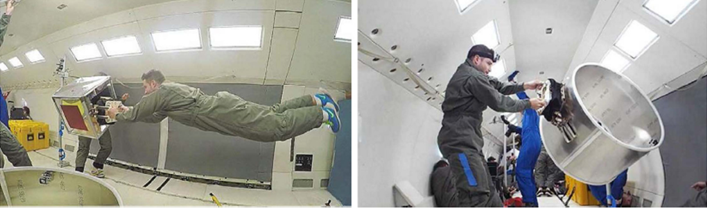
\includegraphics[width=0.7\linewidth]{pics/fly.png}
    \caption{2014 MDA Tests in-flight by ESA}
    \label{fig:fly}
\end{figure}


\subsubsection{ESA Orbit Your Thesis}
The Orbit Your Thesis program extends the parabolic flight concept to long-duration orbital platforms. 
Here, the same fundamental constraints apply with respect to size, weight, and autonomy, 
but the experimental time is vastly increased compared to parabolic flights. 
This enables more systematic testing, including long-term degradation studies, 
radiation exposure experiments, and automated sequences across weeks or months of operation.  

The adaptation requirements for this platform are similar to those of Fly Your Thesis—miniaturization, 
rack compatibility, and robust autonomous operation. 
However, the longer time frame provides opportunities to integrate 
advanced diagnostic routines and self-calibration features within the software. 
The combination of repeatable orbital cycles and extended exposure to the space environment 
makes this a promising platform for bridging ground validation with future operational use in Active Debris Removal missions.

\begin{figure}[h!]
    \centering
    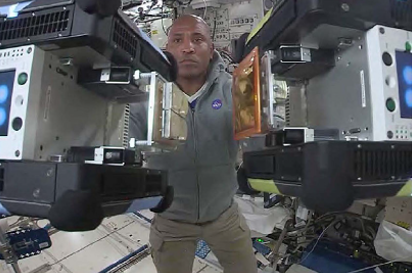
\includegraphics[width=0.7\linewidth]{pics/orbit.png}
    \caption{2020: MDA Tests on the ISS}
    \label{fig:orbit}
\end{figure}

\subsubsection{Bremen Drop Tower}
The Bremen Drop Tower offers highly controlled microgravity conditions for durations between 4.74 and 9.3~seconds, 
depending on whether the catapult mode is used. 
In principle, this facility could be used to test the gecko-inspired adhesion testbed, 
as it provides true free-fall conditions without vibrations or turbulence.  

However, the extremely short time window places significant restrictions on the types of experiments that can be performed. 
Even with optimized control software, a complete adhesion cycle involving approach, contact formation, 
force measurement, and detachment is difficult to achieve within only a few seconds. 
At best, the system could perform a very rapid approach and a preliminary contact test, 
but there would be little opportunity to record high-quality force data or to repeat the experiment for statistical evaluation.  

From an economic perspective, the drop tower is also less attractive compared to parabolic flight campaigns. 
The cost of preparing and executing a drop experiment is high relative to the small amount of usable data that can be collected, 
making it inefficient as a platform for systematic adhesive testing.  

Therefore, while technically possible, the Bremen Drop Tower is not considered a suitable environment for 
comprehensive testing of the gecko adhesion testbed. 
Its role may be limited to quick proof-of-concept demonstrations or rapid-deployment tests, 
but meaningful measurements of adhesion dynamics would require longer-duration platforms such as parabolic flights or orbital missions.


\begin{figure}[h!]
    \centering
    
\includegraphics[width=0.7\linewidth]{pics/bremen.png}
    \caption{Bremen Drop Tower facility with conceptual experiment capsule.}
    \label{fig:bremen}
\end{figure}


In summary, the testbed is inherently scalable across different microgravity platforms, 
with each environment offering specific advantages and limitations. 
Parabolic flights allow repeated testing, orbital missions enable long-term exposure, 
and drop tower experiments deliver clean free-fall conditions. 
Together, these platforms form a progressive pathway for validating gecko-inspired adhesives under increasingly realistic space conditions.


\subsection{Scientific Basis of Gecko-Inspired Adhesion in Space}

The central principle underlying gecko-inspired adhesion is the utilization of van der Waals (vdW) forces, 
which arise from intermolecular interactions at the contact interface between an adhesive surface and its counterpart. 
These forces are quantum-mechanical in nature and act independently of the gravitational field, 
making them fundamentally suitable for application in microgravity environments. 
Unlike suction-based adhesion systems, which depend on ambient pressure differences and are largely ineffective in vacuum, 
vdW adhesion is equally present in space as on Earth.  

Experimental and theoretical studies consistently show that the contact mechanics of micropatterned dry adhesives (MDA) 
are dominated by these van der Waals interactions. 
The magnitude of the adhesive force depends strongly on the effective contact area between the adhesive microstructures 
and the target surface. 
This insight has driven the design of synthetic structures with optimized geometries, 
such as mushroom-shaped terminal features, which maximize real contact area while maintaining the ability to detach cleanly.  
These geometries not only enhance adhesion on smooth surfaces but also improve tolerance to surface irregularities, 
which is essential when considering the heterogeneous surface properties of space debris.  

Another key aspect is that gecko-inspired adhesives are inherently reversible and self-cleaning to some extent. 
Their attachment relies on weak intermolecular interactions rather than chemical bonding or surface damage, 
allowing repeated use without contamination of the substrate. 
This reversibility is highly advantageous for on-orbit servicing and debris removal, 
where multiple docking and detachment operations may be required under varying conditions.  

It is worth noting that earlier debates on potential suction contributions to gecko adhesion have largely been resolved in the context of space. 
Under vacuum conditions, suction plays at most a negligible role, 
and adhesion is overwhelmingly governed by van der Waals forces. 
This understanding reinforces confidence that the observed adhesive performance on Earth can be translated to the orbital environment 
without loss of the underlying physical mechanism.  

\begin{figure}[h!]
    \centering
    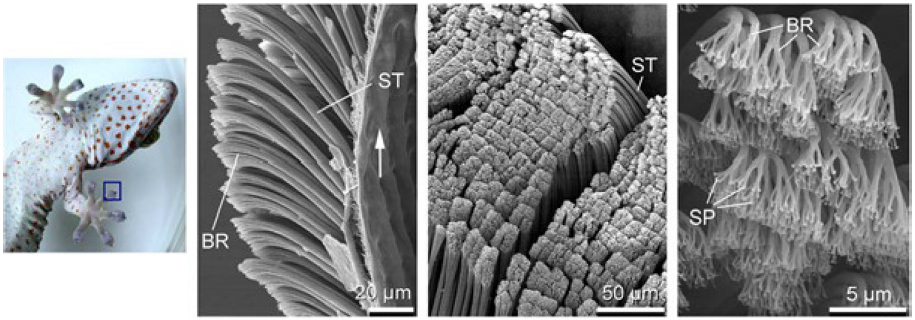
\includegraphics[width=0.7\linewidth]{pics/gecko.png}
    \caption{Adhesive feet of a gecko with a surface, made up of hundreds of thousands of hairs (setae)}
    \label{fig:gecko}
\end{figure}

Taken together, these findings establish a strong scientific foundation for the use of gecko-inspired adhesives in space. 
By relying on van der Waals forces that are unaffected by gravity or atmospheric pressure, 
MDA systems offer a robust and scalable approach for gripping and manipulating objects in orbit. 
The next step lies in evaluating how environmental stressors specific to space, such as radiation and atomic oxygen, 
affect the long-term performance of these materials.


\subsection{Environmental Influences and Open Questions}

While the scientific basis of van der Waals adhesion ensures that the fundamental adhesive forces remain 
effective in microgravity and vacuum, the performance of micropatterned dry adhesives (MDA) 
is still strongly influenced by environmental factors present in space. 
These conditions can alter material properties, surface chemistry, or mechanical stability, 
and therefore must be critically evaluated in the context of orbital applications.  

Radiation represents one of the most significant challenges. 
High-energy particles and ultraviolet radiation are known to induce degradation in many polymeric materials, 
leading to embrittlement, loss of elasticity, and surface cracking. 
For MDA fabricated from polyurethane or similar polymers, 
long-term exposure can reduce adhesion strength by altering the flexibility of the microstructures. 
Preliminary irradiation tests have confirmed a measurable decline in performance after extended radiation doses, 
underscoring the need for either protective coatings or the development of radiation-resistant polymers.  

Thermal cycling in low Earth orbit exposes materials to temperature swings from approximately $-100\,^{\circ}$C to $+100\,^{\circ}$C 
over the course of each orbit. 


\begin{figure}[h!]
    \centering
    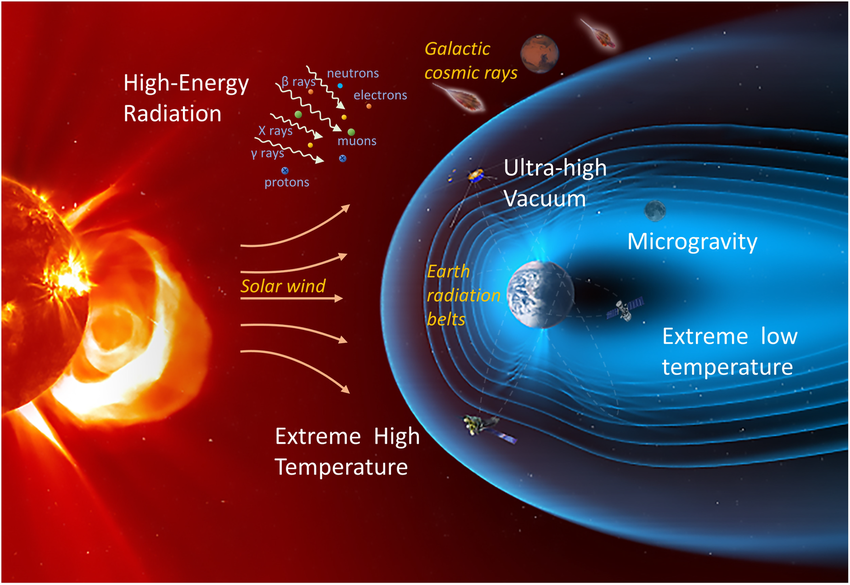
\includegraphics[width=0.7\linewidth]{pics/spaceenv.png}
    \caption{Harsh space environment, affecting the adhesion force of a MDA in the long term.}
    \label{fig:spaceenv}
\end{figure}

Interestingly, adhesion tests conducted under laboratory-controlled thermal variations suggest that 
polyurethane-based adhesives retain their functionality across this range. 
No significant mechanical failures were observed, 
indicating that thermal effects may be less critical than initially assumed. 
Nonetheless, prolonged cycling could induce fatigue in the adhesive backing materials or supporting structures, 
requiring additional investigation.  

Vacuum exposure itself does not diminish van der Waals forces, 
but it can lead to desorption of absorbed water and volatile contaminants from the adhesive surfaces. 
Controlled experiments in vacuum chambers have shown that adhesion values remain largely stable, 
suggesting that this effect is negligible for short-term operations. 
However, multi-month exposure in orbit could still produce subtle changes in surface chemistry that merit attention.  

A particularly critical factor is the presence of atomic oxygen in low Earth orbit. 
Reactive oxygen species are highly erosive and can etch polymer surfaces on a microscopic scale, 
directly degrading the adhesive microstructures that are essential for contact formation. 
Unlike thermal or vacuum effects, atomic oxygen erosion poses a direct threat to the long-term viability of gecko-inspired adhesives. 
Protective surface treatments, such as thin oxide coatings, may be required to mitigate this effect.  

% TODO: Figure suggestion: Table or schematic summarizing key environmental stressors 
% (Radiation, Thermal Cycling, Vacuum, Atomic Oxygen) with arrows showing their impact on adhesion performance.  

In summary, although van der Waals adhesion is fundamentally robust in space, 
the durability of micropatterned dry adhesives depends on the resilience of the underlying material system 
to radiation, atomic oxygen, and cumulative thermal cycling. 
Future research should prioritize long-duration in-situ testing and material optimization 
to ensure that adhesive performance is maintained throughout operational lifetimes in orbit. 
These open questions must be resolved before MDA technology can transition from laboratory demonstrations to real-world space missions.


\subsection{Required Adjustments in Hardware and Software}

Moving the testbed from a laboratory setup to a flight-ready system means that both hardware and software need to be adapted. 
The current version works well on Earth, but it is too large and too dependent on external power and control to be used directly in a microgravity campaign.  

On the hardware side, weight and size are the biggest limitations. 
For parabolic flights, all equipment has to fit into the standardized aircraft racks (about $50 \times 50 \times 80$\,cm). 
This means that actuators, mounting structures, and electronics will need to be redesigned with lighter materials and in a more compact layout. 
Battery power is also essential, since continuous lab power is not available. 
At the same time, the system has to remain mechanically stable and precise enough to run the same adhesion loops that were demonstrated on the ground.  

For the software, the main challenge is autonomy. 
During a parabolic flight there is very little time for manual control, 
so the testbed must be able to recognize the start of the microgravity phase, 
run a full adhesion cycle on its own, and save all data without errors. 
The routines also need to be simple and reliable, because failed cycles mean lost opportunities.  

Finally, the experiments have to be focused. 
In the limited time available it is not possible to test everything, 
so it makes sense to concentrate on patches with different pre-exposures (for example radiation or thermal cycling) 
to compare how these conditions influence adhesion.  


In short, the next step is to make the system smaller, lighter, and fully automatic. 
If these adjustments are achieved, the testbed will be ready to provide useful results 
not only in the lab but also in parabolic flights and, later on, in orbital missions.


\subsection{Outlook}

The gecko-inspired adhesion testbed represents an important step toward advancing bio-inspired gripping 
technologies for space applications. 
Terrestrial experiments have demonstrated that automated, repeatable adhesion testing is feasible with high precision, 
providing a reliable foundation for further development.  

Since gecko-inspired adhesives have already been demonstrated successfully in both parabolic flights 
and orbital experiments, their fundamental suitability for space environments is established. 
The remaining challenge is not proof of principle, but rather the preparation of compact, 
flight-ready test systems that can operate autonomously under strict mass and volume constraints. 
Miniaturization is therefore the key requirement—both for parabolic flight campaigns, 
where size and weight are limited by aircraft rack standards, 
and for orbital missions, where payload capacity and resource efficiency are critical.  

With these adaptations, the testbed could serve as a versatile platform for targeted investigations, 
including long-term material degradation, radiation effects, and repeated adhesion–detachment cycles in orbit. 
Such studies would generate the data needed to qualify micropatterned dry adhesives 
for integration into operational space systems.  

In summary, the immediate focus must shift from demonstrating feasibility—already proven in earlier campaigns— 
towards engineering refinement. 
By achieving lightweight, miniaturized, and autonomous designs, 
the gecko-inspired testbed can transition from a laboratory instrument 
into a practical payload for future parabolic and orbital missions, 
supporting the broader goal of enabling sustainable Active Debris Removal and on-orbit servicing technologies.
\printbibliography

\printglossaries
% Appendix
\appendix
\pagenumbering{roman}
% Manage your appendix
% use \input{appendix/tex_file_name} to add to the appendix

% Project management
\pagebreak
\onecolumn
\begin{landscape}
\section{Project Management}
%______________________________________________________________
% Work Breakdown Structure
% Breakdown of the tasks in individual work packages.
% Up to two levels of workpackages
%______________________________________________________________

\subsection{Work Breakdown Structure}

    \small
    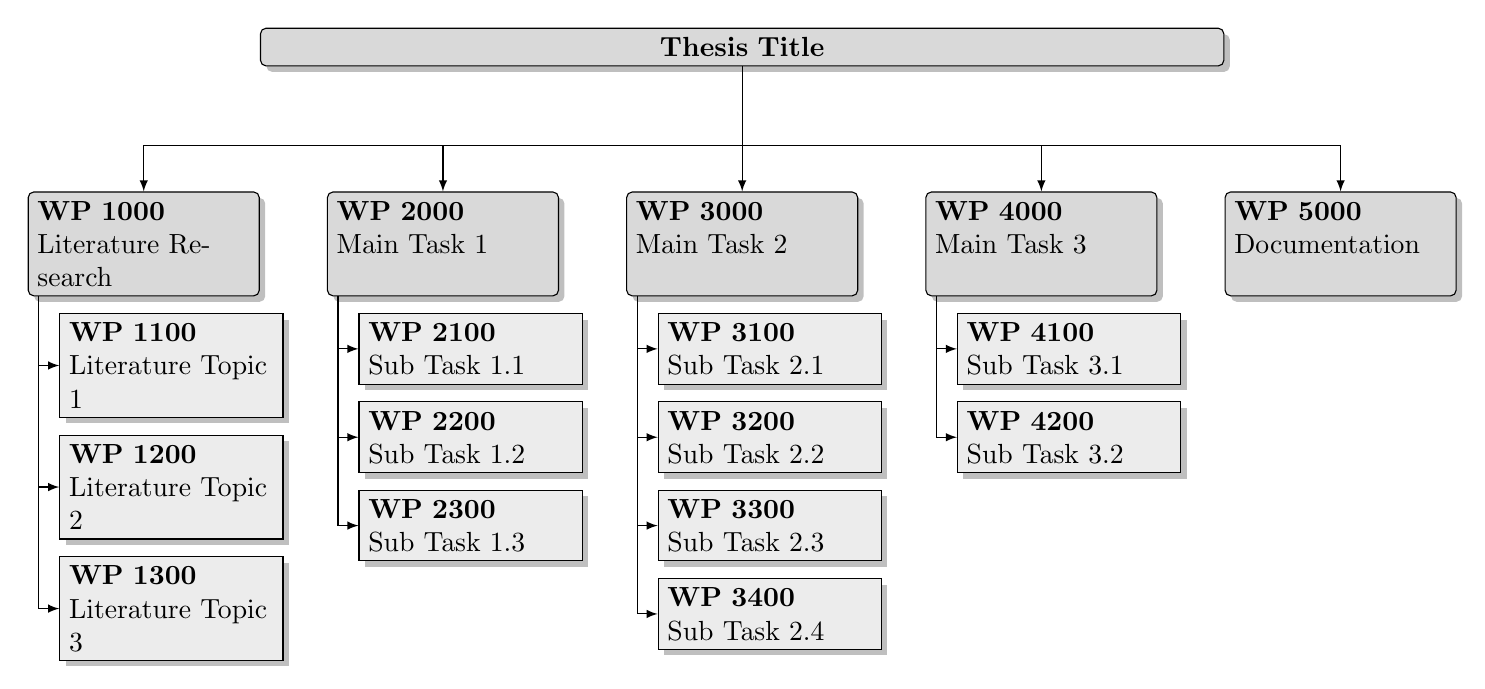
\begin{tikzpicture}[
        basic/.style   = {draw, text width=2.7cm, align=left, drop shadow, rectangle},
        root/.style    = {basic, text width=12cm, rounded corners=2pt, thin, align=center, fill=gray!30},
        level 2/.style = {basic, rounded corners=2pt, thin, fill=gray!30},
        level 3/.style = {basic, thin, fill=gray!15, text width=2.6cm},
        level 1/.style={sibling distance=38mm}, edge from parent fork down,
        edge from parent/.style={->,draw}, level distance=2.5cm,  >=latex]

    % root of the the initial tree, level 1
    \node[root] {\textbf{Thesis Title}}
    % The first level, as children of the initial tree
        child {node[level 2] (c1) {\textbf{WP~1000} \\ Literature Research}}
        child {node[level 2] (c2) {\textbf{WP~2000} \\ Main Task 1 \\ $~~$}}
        child {node[level 2] (c3) {\textbf{WP~3000} \\ Main Task 2 \\ $~~$}}
        child {node[level 2] (c4) {\textbf{WP~4000} \\ Main Task 3 \\ $~~$}}
        child {node[level 2] (c5) {\textbf{WP~5000} \\ Documentation \\ $~~$}};

    % The second level, relatively positioned nodes
    \begin{scope}[every node/.style={level 3}, node distance=6pt]
    \node [below=of c1, xshift=10pt] (c11) {\textbf{WP~1100} \\ Literature Topic 1};
    \node [below=of c11] (c12) {\textbf{WP~1200} \\ Literature Topic 2};
    \node [below=of c12] (c13) {\textbf{WP~1300} \\ Literature Topic 3};

    \node [below=of c2, xshift=10pt] (c21) {\textbf{WP~2100} \\ Sub Task 1.1};
    \node [below=of c21] (c22) {\textbf{WP~2200} \\ Sub Task 1.2};
    \node [below=of c22] (c23) {\textbf{WP~2300} \\ Sub Task 1.3};

    \node [below=of c3, xshift=10pt] (c31) {\textbf{WP~3100} \\ Sub Task 2.1};
    \node [below=of c31] (c32) {\textbf{WP~3200} \\ Sub Task 2.2};
    \node [below=of c32] (c33) {\textbf{WP~3300} \\ Sub Task 2.3};
    \node [below=of c33] (c34) {\textbf{WP~3400} \\ Sub Task 2.4};

    \node [below=of c4, xshift=10pt] (c41) {\textbf{WP~4100} \\ Sub Task 3.1};
    \node [below=of c41] (c42) {\textbf{WP~4200} \\ Sub Task 3.2};

    \end{scope}

    % lines from each level 1 node to every one of its "children"
    \foreach \value in {1,2,3}
        \draw[->] ([xshift=4pt]c1.south west) |- (c1\value.west);

    \foreach \value in {1,2,3}
        \draw[->] ([xshift=4pt]c2.south west) |- (c2\value.west);

    \foreach \value in {1,2,3,4}
        \draw[->] ([xshift=4pt]c3.south west) |- (c3\value.west);

    \foreach \value in {1,2}
        \draw[->] ([xshift=4pt]c4.south west) |- (c4\value.west);

    \end{tikzpicture}
    \normalsize

\end{landscape}

\begin{landscape}

%______________________________________________________________
% Gantt Chart
% Time line of the project
% Shows duration and chronological structure for each 
%  workpackage and project milestones
%______________________________________________________________
\subsection{Gantt Chart}
\definecolor{color_bar}{RGB}{0, 63, 137}
\definecolor{color_group}{RGB}{0, 37, 82}
\begin{center}
    \begin{ganttchart}[
        expand chart=.95\linewidth,
        vgrid,
        bar/.append style={fill=color_bar, draw=none},
        group/.append style={fill=color_group},
        group left shift=0,
        group right shift=0,
        group peaks tip position=0,
        group peaks height=.25,
        y unit chart = 0.445cm,
        group top shift=0.25,
        bar top shift=-0.1,
        bar height=0.6,
        milestone top shift=-0.1,
        milestone/.append style={xscale=0.5}]{1}{16}
        \gantttitle{Weeks}{16} \\
        \gantttitlelist{1,...,16}{1} \\

        \ganttgroup{WP 1000: Literature Research}{1}{5} \\
        \ganttbar{WP 1100: Literature Topic 1}{1}{3} \\
        \ganttbar{WP 1200: Literature Topic 2}{2}{4} \\
        \ganttbar{WP 1300: Literature Topic 3}{2}{5} \\
        \\
        \ganttgroup{WP 2000: Main Task 1}{4}{8} \\
        \ganttbar{WP 2100: Sub Task 1.1}{4}{6} \\
        \ganttbar{WP 2200: Sub Task 1.2}{6}{7} \\
        \ganttbar{WP 2300: Sub Task 1.3}{7}{8} \\
        \ganttmilestone{Milestone 1}{8} \\
        \\
        \ganttgroup{WP 3000: Main Task 2}{4}{11} \\
        \ganttbar{WP 3100: Sub Task 2.1}{4}{5} \\
        \ganttbar{WP 3200: Sub Task 2.2}{5}{6} \\
        \ganttbar{WP 3300: Sub Task 2.3}{6}{8} \\
        \ganttbar{WP 3400: Sub Task 2.4}{7}{11} \\
        \ganttmilestone{Milestone 2}{11} \\
        \\
        \ganttgroup{WP 4000: Main Task 3}{8}{12} \\
        \ganttbar{WP 4100: Sub Task 3.1}{8}{12} \\
        \ganttbar{WP 4200: Sub Task 3.2}{8}{12} \\
        \ganttmilestone{Milestone 3}{12} \\
        \\
        \ganttgroup{WP 5000: Documentation}{1}{16} \\
        \ganttmilestone{Draft}{12} \\
        \ganttmilestone{Submission}{16}
    \end{ganttchart}
\end{center}
\end{landscape}

%______________________________________________________________
% Work Package Description
% Detailed description of each workpackage
%______________________________________________________________

\subsection{Work Package Description}

\newcommand{\wpddate}{27.09.2021}
%%%%
% WP1000 - Literature Research
%%%%

\begin{table}[!h]
    \begin{center}
        \begin{tabular}{|p{.2\columnwidth}||p{.3\columnwidth}|p{.27\columnwidth}||p{.23\columnwidth}|}
            \hline
            \multicolumn{3}{|l||}{\textbf{}} & \multicolumn{1}{c|}{}\\
            \multicolumn{3}{|l||}{\textbf{}} & \multicolumn{1}{c|}{\textbf{WP 1100}}\\
            \multicolumn{3}{|l||}{\textbf{}} & \multicolumn{1}{c|}{}\\
            \hline\hline
            \textbf{Title} & \multicolumn{2}{p{.40\columnwidth}||}{\textbf{Literature Topic 1}}
            & \textbf{Page:} 1 of 1\\
            \hline
            \textbf{Responsible} & \multicolumn{2}{l||}{Ame Watson} & \textbf{Version:} 1.0\\
            \hline
            \multicolumn{3}{|l||}{} & \textbf{Date:} \wpddate\\
            \hline\hline
            \textbf{Start} & \multicolumn{2}{l||}{Week 1} & \\
            \hline
            \textbf{End} & \multicolumn{2}{l||}{Week 3} & \textbf{Duration}: 3 Weeks\\
            \hline\hline
            \textbf{Processed by} & \multicolumn{3}{l|}{Ame Watson}\\
            \hline\hline
            \multicolumn{4}{|p{.95\columnwidth}|}{\textbf{Goals:}}\\
            \multicolumn{4}{|p{.95\columnwidth}|}{$\bullet$ Gain knowledge about the literature research topic 1}\\
            \multicolumn{4}{|p{.95\columnwidth}|}{$\bullet$ Gain a deep understanding of the current state of the art on research topic 1}\\
            \multicolumn{4}{|p{.95\columnwidth}|}{}\\
            \multicolumn{4}{|p{.95\columnwidth}|}{\textbf{Input:}}\\
            \multicolumn{4}{|p{.95\columnwidth}|}{$\bullet$ Journal papers on literature topic 1}\\
            \multicolumn{4}{|p{.95\columnwidth}|}{$\bullet$ Conference papers on literature topic 1}\\
            \multicolumn{4}{|p{.95\columnwidth}|}{}\\
            \multicolumn{4}{|p{.95\columnwidth}|}{\textbf{Connections to other WPs:}}\\
            \multicolumn{4}{|p{.95\columnwidth}|}{}\\
            \multicolumn{4}{|p{.95\columnwidth}|}{\textbf{Tasks:}}\\
            \multicolumn{4}{|p{.95\columnwidth}|}{$\bullet$ Literature research literature topic 1}\\
            \multicolumn{4}{|p{.95\columnwidth}|}{}\\
            \multicolumn{4}{|p{.95\columnwidth}|}{\textbf{Results:}}\\
            \multicolumn{4}{|p{.95\columnwidth}|}{$\bullet$ Basic knowledge about literature topic 1}\\
            \multicolumn{4}{|p{.95\columnwidth}|}{$\bullet$ Deeper knowledge about literature topic 1}\\
            \hline
        \end{tabular}
    \end{center}
\end{table}

\clearpage

\begin{table}[!h]
    \begin{center}
        \begin{tabular}{|p{.2\columnwidth}||p{.3\columnwidth}|p{.27\columnwidth}||p{.23\columnwidth}|}
            \hline
            \multicolumn{3}{|l||}{\textbf{}} & \multicolumn{1}{c|}{}\\
            \multicolumn{3}{|l||}{\textbf{}} & \multicolumn{1}{c|}{\textbf{WP 1200}}\\
            \multicolumn{3}{|l||}{\textbf{}} & \multicolumn{1}{c|}{}\\
            \hline\hline
            \textbf{Title} & \multicolumn{2}{p{.40\columnwidth}||}{\textbf{Literature Topic 2}}
            & \textbf{Page:} 1 of 1\\
            \hline
            \textbf{Responsible} & \multicolumn{2}{l||}{Ame Watson} & \textbf{Version:} 1.0\\
            \hline
            \multicolumn{3}{|l||}{} & \textbf{Date:} \wpddate\\
            \hline\hline
            \textbf{Start} & \multicolumn{2}{l||}{Week 2} & \\
            \hline
            \textbf{End} & \multicolumn{2}{l||}{Week 4} & \textbf{Duration}: 3 Weeks\\
            \hline\hline
            \textbf{Processed by} & \multicolumn{3}{l|}{Ame Watson}\\
            \hline\hline
            \multicolumn{4}{|p{.95\columnwidth}|}{\textbf{Goals:}}\\
            \multicolumn{4}{|p{.95\columnwidth}|}{$\bullet$ Get insight into literature topic 2}\\
            \multicolumn{4}{|p{.95\columnwidth}|}{$\bullet$ Gather state-of-the-art information on literature topic 2}\\
            \multicolumn{4}{|p{.95\columnwidth}|}{}\\
            \multicolumn{4}{|p{.95\columnwidth}|}{\textbf{Input:}}\\
            \multicolumn{4}{|p{.95\columnwidth}|}{$\bullet$ Literature on literature topic 2}\\
            \multicolumn{4}{|p{.95\columnwidth}|}{$\bullet$ Literature on literature topic 2}\\
            \multicolumn{4}{|p{.95\columnwidth}|}{}\\
            \multicolumn{4}{|p{.95\columnwidth}|}{\textbf{Connections to other WPs:}}\\
            \multicolumn{4}{|p{.95\columnwidth}|}{}\\
            \multicolumn{4}{|p{.95\columnwidth}|}{\textbf{Tasks:}}\\
            \multicolumn{4}{|p{.95\columnwidth}|}{$\bullet$ Literature research on literature topic 2}\\
            \multicolumn{4}{|p{.95\columnwidth}|}{$\bullet$ Literature research on literature topic 2}\\
            \multicolumn{4}{|p{.95\columnwidth}|}{}\\
            \multicolumn{4}{|p{.95\columnwidth}|}{\textbf{Results:}}\\
            \multicolumn{4}{|p{.95\columnwidth}|}{$\bullet$ Basic knowledge on literature topic 2}\\
            \multicolumn{4}{|p{.95\columnwidth}|}{$\bullet$ Basic knowledge on literature topic 2 in general}\\
            \hline
        \end{tabular}
    \end{center}
\end{table}

\clearpage

\begin{table}[!h]
    \begin{center}
        \begin{tabular}{|p{.2\columnwidth}||p{.3\columnwidth}|p{.27\columnwidth}||p{.23\columnwidth}|}
            \hline
            \multicolumn{3}{|l||}{\textbf{}} & \multicolumn{1}{c|}{}\\
            \multicolumn{3}{|l||}{\textbf{}} & \multicolumn{1}{c|}{\textbf{WP 1300}}\\
            \multicolumn{3}{|l||}{\textbf{}} & \multicolumn{1}{c|}{}\\
            \hline\hline
            \textbf{Title} & \multicolumn{2}{p{.40\columnwidth}||}{\textbf{Literature Topic 3}}
            & \textbf{Page:} 1 of 1\\
            \hline
            \textbf{Responsible} & \multicolumn{2}{l||}{Ame Watson} & \textbf{Version:} 1.0\\
            \hline
            \multicolumn{3}{|l||}{} & \textbf{Date:} \wpddate\\
            \hline\hline
            \textbf{Start} & \multicolumn{2}{l||}{Week 2} & \\
            \hline
            \textbf{End} & \multicolumn{2}{l||}{Week 5} & \textbf{Duration}: 4 Weeks\\
            \hline\hline
            \textbf{Processed by} & \multicolumn{3}{l|}{Ame Watson}\\
            \hline\hline
            \multicolumn{4}{|p{.95\columnwidth}|}{\textbf{Goals:}}\\
            \multicolumn{4}{|p{.95\columnwidth}|}{$\bullet$ Get insight into literature topic 3, to be able to derive decisions and requirements about stuff}\\
            \multicolumn{4}{|p{.95\columnwidth}|}{}\\
            \multicolumn{4}{|p{.95\columnwidth}|}{\textbf{Input:}}\\
            \multicolumn{4}{|p{.95\columnwidth}|}{$\bullet$ Documentation of literature topic 3}\\
            \multicolumn{4}{|p{.95\columnwidth}|}{}\\
            \multicolumn{4}{|p{.95\columnwidth}|}{\textbf{Connections to other WPs:}}\\
            \multicolumn{4}{|p{.95\columnwidth}|}{$\bullet$ \textbf{WP 3200} Research for subsystems/units/parts/components}\\
            \multicolumn{4}{|p{.95\columnwidth}|}{$\bullet$ \textbf{WP 3200} Gather technical solutions for novel design}\\
            \multicolumn{4}{|p{.95\columnwidth}|}{}\\
            \multicolumn{4}{|p{.95\columnwidth}|}{\textbf{Tasks:}}\\
            \multicolumn{4}{|p{.95\columnwidth}|}{$\bullet$ Literature research on literature topic 3}\\            \multicolumn{4}{|p{.95\columnwidth}|}{}\\
            \multicolumn{4}{|p{.95\columnwidth}|}{\textbf{Results:}}\\
            \multicolumn{4}{|p{.95\columnwidth}|}{$\bullet$ Select technical solutions of literature topic 3 as proposal for thingy to be developed}\\
            \hline
        \end{tabular}
    \end{center}
\end{table}

\clearpage

%%%%
% WP2000 - Main Task 1
%%%%

\begin{table}[!h]
    \begin{center}
        \begin{tabular}{|p{.2\columnwidth}||p{.3\columnwidth}|p{.27\columnwidth}||p{.23\columnwidth}|}
            \hline
            \multicolumn{3}{|l||}{\textbf{}} & \multicolumn{1}{c|}{}\\
            \multicolumn{3}{|l||}{\textbf{}} & \multicolumn{1}{c|}{\textbf{WP 2100}}\\
            \multicolumn{3}{|l||}{\textbf{}} & \multicolumn{1}{c|}{}\\
            \hline\hline
            \textbf{Title} & \multicolumn{2}{p{.40\columnwidth}||}{\textbf{Sub Task 1.1}}
            & \textbf{Page:} 1 of 1\\
            \hline
            \textbf{Responsible} & \multicolumn{2}{l||}{Ame Watson} & \textbf{Version:} 1.0\\
            \hline
            \multicolumn{3}{|l||}{} & \textbf{Date:} \wpddate\\
            \hline\hline
            \textbf{Start} & \multicolumn{2}{l||}{Week 4} & \\
            \hline
            \textbf{End} & \multicolumn{2}{l||}{Week 6} & \textbf{Duration}: 3 Weeks\\
            \hline\hline
            \textbf{Processed by} & \multicolumn{3}{l|}{Ame Watson}\\
            \hline\hline
            \multicolumn{4}{|p{.95\columnwidth}|}{\textbf{Goals:}}\\
            \multicolumn{4}{|p{.95\columnwidth}|}{$\bullet$ Identify needs and characteristics for sub task 2.1}\\
            \multicolumn{4}{|p{.95\columnwidth}|}{$\bullet$ Identify requirements and expected performance}\\
            \multicolumn{4}{|p{.95\columnwidth}|}{$\bullet$ Identify constraints}\\
            \multicolumn{4}{|p{.95\columnwidth}|}{}\\
            \multicolumn{4}{|p{.95\columnwidth}|}{\textbf{Input:}}\\
            \multicolumn{4}{|p{.95\columnwidth}|}{$\bullet$ Documentation, haha }\\
            \multicolumn{4}{|p{.95\columnwidth}|}{$\bullet$ Documentation of other stuff xD}\\
            \multicolumn{4}{|p{.95\columnwidth}|}{}\\
            \multicolumn{4}{|p{.95\columnwidth}|}{\textbf{Connections to other WPs:}}\\
            \multicolumn{4}{|p{.95\columnwidth}|}{$\bullet$ \textbf{WP 1100} Input from the literature research}\\
            \multicolumn{4}{|p{.95\columnwidth}|}{}\\
            \multicolumn{4}{|p{.95\columnwidth}|}{\textbf{Tasks:}}\\
            \multicolumn{4}{|p{.95\columnwidth}|}{$\bullet$ Precisely define the thingy to be defined in sub task 2.1}\\
            \multicolumn{4}{|p{.95\columnwidth}|}{}\\
            \multicolumn{4}{|p{.95\columnwidth}|}{\textbf{Results:}}\\
            \multicolumn{4}{|p{.95\columnwidth}|}{$\bullet$ Requirements for development thingy}\\
            \multicolumn{4}{|p{.95\columnwidth}|}{$\bullet$ Furhter results}\\
            \hline
        \end{tabular}
    \end{center}
\end{table}

\clearpage

\begin{table}[!h]
    \begin{center}
        \begin{tabular}{|p{.2\columnwidth}||p{.3\columnwidth}|p{.27\columnwidth}||p{.23\columnwidth}|}
            \hline
            \multicolumn{3}{|l||}{\textbf{}} & \multicolumn{1}{c|}{}\\
            \multicolumn{3}{|l||}{\textbf{}} & \multicolumn{1}{c|}{\textbf{WP 2200}}\\
            \multicolumn{3}{|l||}{\textbf{}} & \multicolumn{1}{c|}{}\\
            \hline\hline
            \textbf{Title} & \multicolumn{2}{p{.40\columnwidth}||}{\textbf{Sub Task 1.2}}
            & \textbf{Page:} 1 of 1\\
            \hline
            \textbf{Responsible} & \multicolumn{2}{l||}{Ame Watson} & \textbf{Version:} 1.0\\
            \hline
            \multicolumn{3}{|l||}{} & \textbf{Date:} \wpddate\\
            \hline\hline
            \textbf{Start} & \multicolumn{2}{l||}{Week 6} & \\
            \hline
            \textbf{End} & \multicolumn{2}{l||}{Week 7} & \textbf{Duration}: 2 Weeks\\
            \hline\hline
            \textbf{Processed by} & \multicolumn{3}{l|}{Ame Watson}\\
            \hline\hline
            \multicolumn{4}{|p{.95\columnwidth}|}{\textbf{Goals:}}\\
            \multicolumn{4}{|p{.95\columnwidth}|}{$\bullet$ Compare the current state of the stuff to the previous defined requirements}\\
            \multicolumn{4}{|p{.95\columnwidth}|}{$\bullet$ Additional Goal}\\
            \multicolumn{4}{|p{.95\columnwidth}|}{}\\
            \multicolumn{4}{|p{.95\columnwidth}|}{\textbf{Input:}}\\
            \multicolumn{4}{|p{.95\columnwidth}|}{$\bullet$ Results from WPXXXX}\\
            \multicolumn{4}{|p{.95\columnwidth}|}{$\bullet$ Input from WPXXXX}\\
            \multicolumn{4}{|p{.95\columnwidth}|}{}\\
            \multicolumn{4}{|p{.95\columnwidth}|}{\textbf{Connections to other WPs:}}\\
            \multicolumn{4}{|p{.95\columnwidth}|}{$\bullet$ \textbf{WP XXXX} Connection to this workpkg}\\
            \multicolumn{4}{|p{.95\columnwidth}|}{$\bullet$ \textbf{WP XXXX} Connection to this workpkg}\\
            \multicolumn{4}{|p{.95\columnwidth}|}{}\\
            \multicolumn{4}{|p{.95\columnwidth}|}{\textbf{Tasks:}}\\
            \multicolumn{4}{|p{.95\columnwidth}|}{$\bullet$ Task-A of Sub Task 1.2}\\
            \multicolumn{4}{|p{.95\columnwidth}|}{$\bullet$ Task-B of Sub Task 1.2}\\
            \multicolumn{4}{|p{.95\columnwidth}|}{}\\
            \multicolumn{4}{|p{.95\columnwidth}|}{\textbf{Results:}}\\
            \multicolumn{4}{|p{.95\columnwidth}|}{$\bullet$ Result of Sub Task 1.2}\\
            \hline
        \end{tabular}
    \end{center}
\end{table}

\clearpage

\begin{table}[!h]
    \begin{center}
        \begin{tabular}{|p{.2\columnwidth}||p{.3\columnwidth}|p{.27\columnwidth}||p{.23\columnwidth}|}
            \hline
            \multicolumn{3}{|l||}{\textbf{}} & \multicolumn{1}{c|}{}\\
            \multicolumn{3}{|l||}{\textbf{}} & \multicolumn{1}{c|}{\textbf{WP 2300}}\\
            \multicolumn{3}{|l||}{\textbf{}} & \multicolumn{1}{c|}{}\\
            \hline\hline
            \textbf{Title} & \multicolumn{2}{p{.40\columnwidth}||}{\textbf{Sub Task 1.3}}
            & \textbf{Page:} 1 of 1\\
            \hline
            \textbf{Responsible} & \multicolumn{2}{l||}{Ame Watson} & \textbf{Version:} 1.0\\
            \hline
            \multicolumn{3}{|l||}{} & \textbf{Date:} \wpddate\\
            \hline\hline
            \textbf{Start} & \multicolumn{2}{l||}{Week 6} & \\
            \hline
            \textbf{End} & \multicolumn{2}{l||}{Week 8} & \textbf{Duration}: 2 Weeks\\
            \hline\hline
            \textbf{Processed by} & \multicolumn{3}{l|}{Ame Watson}\\
            \hline\hline
            \multicolumn{4}{|p{.95\columnwidth}|}{\textbf{Goals:}}\\
            \multicolumn{4}{|p{.95\columnwidth}|}{$\bullet$ Goal-A of Sub Task 1.3}\\
            \multicolumn{4}{|p{.95\columnwidth}|}{$\bullet$ Goal-B of Sub Task 1.3}\\
            \multicolumn{4}{|p{.95\columnwidth}|}{}\\
            \multicolumn{4}{|p{.95\columnwidth}|}{\textbf{Input:}}\\
            \multicolumn{4}{|p{.95\columnwidth}|}{$\bullet$ Results from WPXXXX}\\
            \multicolumn{4}{|p{.95\columnwidth}|}{$\bullet$ Input from WPXXXX}\\
            \multicolumn{4}{|p{.95\columnwidth}|}{}\\
            \multicolumn{4}{|p{.95\columnwidth}|}{\textbf{Connections to other WPs:}}\\
            \multicolumn{4}{|p{.95\columnwidth}|}{$\bullet$ \textbf{WP XXXX} connection to this workpg}\\
            \multicolumn{4}{|p{.95\columnwidth}|}{$\bullet$ \textbf{WP XXXX} connection to this workpg}\\
            \multicolumn{4}{|p{.95\columnwidth}|}{}\\
            \multicolumn{4}{|p{.95\columnwidth}|}{\textbf{Tasks:}}\\
            \multicolumn{4}{|p{.95\columnwidth}|}{$\bullet$ Task-A of Sub Task 1.3}\\
            \multicolumn{4}{|p{.95\columnwidth}|}{$\bullet$ Task-B of Sub Task 1.3}\\
            \multicolumn{4}{|p{.95\columnwidth}|}{}\\
            \multicolumn{4}{|p{.95\columnwidth}|}{\textbf{Results:}}\\
            \multicolumn{4}{|p{.95\columnwidth}|}{$\bullet$ Result of Sub Task 1.3}\\
            \hline
        \end{tabular}
    \end{center}
\end{table}

\clearpage

%%%%
% WP3000 - Main Task 2
%%%%

\begin{table}[!h]
    \begin{center}
        \begin{tabular}{|p{.2\columnwidth}||p{.3\columnwidth}|p{.27\columnwidth}||p{.23\columnwidth}|}
            \hline
            \multicolumn{3}{|l||}{\textbf{}} & \multicolumn{1}{c|}{}\\
            \multicolumn{3}{|l||}{\textbf{}} & \multicolumn{1}{c|}{\textbf{WP 3100}}\\
            \multicolumn{3}{|l||}{\textbf{}} & \multicolumn{1}{c|}{}\\
            \hline\hline
            \textbf{Title} & \multicolumn{2}{p{.40\columnwidth}||}{\textbf{Sub Task 2.1}}
            & \textbf{Page:} 1 of 1\\
            \hline
            \textbf{Responsible} & \multicolumn{2}{l||}{Ame Watson} & \textbf{Version:} 1.0\\
            \hline
            \multicolumn{3}{|l||}{} & \textbf{Date:} \wpddate\\
            \hline\hline
            \textbf{Start} & \multicolumn{2}{l||}{Week 4} & \\
            \hline
            \textbf{End} & \multicolumn{2}{l||}{Week 5} & \textbf{Duration}: 2 Weeks\\
            \hline\hline
            \textbf{Processed by} & \multicolumn{3}{l|}{Ame Watson}\\
            \hline\hline
            \multicolumn{4}{|p{.95\columnwidth}|}{\textbf{Goals:}}\\
            \multicolumn{4}{|p{.95\columnwidth}|}{$\bullet$ Goal of Sub Task 2.1}\\
            \multicolumn{4}{|p{.95\columnwidth}|}{}\\
            \multicolumn{4}{|p{.95\columnwidth}|}{\textbf{Input:}}\\
            \multicolumn{4}{|p{.95\columnwidth}|}{$\bullet$ Input-A for Sub Task 2.1}\\
            \multicolumn{4}{|p{.95\columnwidth}|}{$\bullet$ Input-B for Sub Task 2.1}\\
            \multicolumn{4}{|p{.95\columnwidth}|}{$\bullet$ Input-C for Sub Task 2.1}\\
            \multicolumn{4}{|p{.95\columnwidth}|}{}\\
            \multicolumn{4}{|p{.95\columnwidth}|}{\textbf{Connections to other WPs:}}\\
            \multicolumn{4}{|p{.95\columnwidth}|}{$\bullet$ \textbf{WP XXXX} connection to this workpkg}\\
            \multicolumn{4}{|p{.95\columnwidth}|}{$\bullet$ \textbf{WP XXXX} connection to this workpkg}\\
            \multicolumn{4}{|p{.95\columnwidth}|}{$\bullet$ \textbf{WP XXXX} connection to this workpkg}\\
            \multicolumn{4}{|p{.95\columnwidth}|}{}\\
            \multicolumn{4}{|p{.95\columnwidth}|}{\textbf{Tasks:}}\\
            \multicolumn{4}{|p{.95\columnwidth}|}{$\bullet$ Task of Sub Task 2.1}\\
            \multicolumn{4}{|p{.95\columnwidth}|}{}\\
            \multicolumn{4}{|p{.95\columnwidth}|}{\textbf{Results:}}\\
            \multicolumn{4}{|p{.95\columnwidth}|}{$\bullet$ Result-A of Sub Task 2.1}\\
            \multicolumn{4}{|p{.95\columnwidth}|}{$\bullet$ Result-B of Sub Task 2.1}\\
            \hline
        \end{tabular}
    \end{center}
\end{table}

\clearpage

\begin{table}[!h]
    \begin{center}
        \begin{tabular}{|p{.2\columnwidth}||p{.3\columnwidth}|p{.27\columnwidth}||p{.23\columnwidth}|}
            \hline
            \multicolumn{3}{|l||}{\textbf{}} & \multicolumn{1}{c|}{}\\
            \multicolumn{3}{|l||}{\textbf{}} & \multicolumn{1}{c|}{\textbf{WP 3200}}\\
            \multicolumn{3}{|l||}{\textbf{}} & \multicolumn{1}{c|}{}\\
            \hline\hline
            \textbf{Title} & \multicolumn{2}{p{.40\columnwidth}||}{\textbf{Sub Task 2.2}}
            & \textbf{Page:} 1 of 1\\
            \hline
            \textbf{Responsible} & \multicolumn{2}{l||}{Ame Watson} & \textbf{Version:} 1.0\\
            \hline
            \multicolumn{3}{|l||}{} & \textbf{Date:} \wpddate\\
            \hline\hline
            \textbf{Start} & \multicolumn{2}{l||}{Week 5} & \\
            \hline
            \textbf{End} & \multicolumn{2}{l||}{Week 6} & \textbf{Duration}: 2 Weeks\\
            \hline\hline
            \textbf{Processed by} & \multicolumn{3}{l|}{Ame Watson}\\
            \hline\hline
            \multicolumn{4}{|p{.95\columnwidth}|}{\textbf{Goals:}}\\
            \multicolumn{4}{|p{.95\columnwidth}|}{$\bullet$ Goal-A of Sub Task 2.2}\\
            \multicolumn{4}{|p{.95\columnwidth}|}{$\bullet$ Goal-B of Sub Task 2.2}\\
            \multicolumn{4}{|p{.95\columnwidth}|}{}\\
            \multicolumn{4}{|p{.95\columnwidth}|}{\textbf{Input:}}\\
            \multicolumn{4}{|p{.95\columnwidth}|}{$\bullet$ Input-A for Sub Task 2.2}\\
            \multicolumn{4}{|p{.95\columnwidth}|}{$\bullet$ Input-B for Sub Task 2.2}\\
            \multicolumn{4}{|p{.95\columnwidth}|}{}\\
            \multicolumn{4}{|p{.95\columnwidth}|}{\textbf{Connections to other WPs:}}\\
            \multicolumn{4}{|p{.95\columnwidth}|}{$\bullet$ \textbf{WP XXXX/XXXX} connection to these workpkgs}\\
            \multicolumn{4}{|p{.95\columnwidth}|}{$\bullet$ \textbf{WP XXXX/XXXX} connection to these workpkgs}\\
            \multicolumn{4}{|p{.95\columnwidth}|}{}\\
            \multicolumn{4}{|p{.95\columnwidth}|}{\textbf{Tasks:}}\\
            \multicolumn{4}{|p{.95\columnwidth}|}{$\bullet$ Task-A of Sub Task 2.2}\\
            \multicolumn{4}{|p{.95\columnwidth}|}{$\bullet$ Task-B of Sub Task 2.2}\\
            \multicolumn{4}{|p{.95\columnwidth}|}{}\\
            \multicolumn{4}{|p{.95\columnwidth}|}{\textbf{Results:}}\\
            \multicolumn{4}{|p{.95\columnwidth}|}{$\bullet$ Result-A of Sub Task 2.2}\\
            \multicolumn{4}{|p{.95\columnwidth}|}{$\bullet$ Result-B of Sub Task 2.2}\\
            \hline
        \end{tabular}
    \end{center}
\end{table}

\clearpage

\begin{table}[!h]
    \begin{center}
        \begin{tabular}{|p{.2\columnwidth}||p{.3\columnwidth}|p{.27\columnwidth}||p{.23\columnwidth}|}
            \hline
            \multicolumn{3}{|l||}{\textbf{}} & \multicolumn{1}{c|}{}\\
            \multicolumn{3}{|l||}{\textbf{}} & \multicolumn{1}{c|}{\textbf{WP 3300}}\\
            \multicolumn{3}{|l||}{\textbf{}} & \multicolumn{1}{c|}{}\\
            \hline\hline
            \textbf{Title} & \multicolumn{2}{p{.40\columnwidth}||}{\textbf{Sub Task 2.3}}
            & \textbf{Page:} 1 of 1\\
            \hline
            \textbf{Responsible} & \multicolumn{2}{l||}{Ame Watson} & \textbf{Version:} 1.0\\
            \hline
            \multicolumn{3}{|l||}{} & \textbf{Date:} \wpddate\\
            \hline\hline
            \textbf{Start} & \multicolumn{2}{l||}{Week 6} & \\
            \hline
            \textbf{End} & \multicolumn{2}{l||}{Week 8} & \textbf{Duration}: 3 Weeks\\
            \hline\hline
            \textbf{Processed by} & \multicolumn{3}{l|}{Ame Watson}\\
            \hline\hline
            \multicolumn{4}{|p{.95\columnwidth}|}{\textbf{Goals:}}\\
            \multicolumn{4}{|p{.95\columnwidth}|}{$\bullet$ Goal of Sub Task 2.3}\\
            \multicolumn{4}{|p{.95\columnwidth}|}{}\\
            \multicolumn{4}{|p{.95\columnwidth}|}{\textbf{Input:}}\\
            \multicolumn{4}{|p{.95\columnwidth}|}{$\bullet$ Input for Sub Task 2.1}\\
            \multicolumn{4}{|p{.95\columnwidth}|}{}\\
            \multicolumn{4}{|p{.95\columnwidth}|}{\textbf{Connections to other WPs:}}\\
            \multicolumn{4}{|p{.95\columnwidth}|}{}\\
            \multicolumn{4}{|p{.95\columnwidth}|}{\textbf{Tasks:}}\\
            \multicolumn{4}{|p{.95\columnwidth}|}{$\bullet$ Task of Sub Task 2.3}\\
            \multicolumn{4}{|p{.95\columnwidth}|}{}\\
            \multicolumn{4}{|p{.95\columnwidth}|}{\textbf{Results:}}\\
            \multicolumn{4}{|p{.95\columnwidth}|}{$\bullet$ Result of Sub Task 2.3}\\
            \hline
        \end{tabular}
    \end{center}
\end{table}

\clearpage

\begin{table}[!h]
    \begin{center}
        \begin{tabular}{|p{.2\columnwidth}||p{.3\columnwidth}|p{.27\columnwidth}||p{.23\columnwidth}|}
            \hline
            \multicolumn{3}{|l||}{\textbf{}} & \multicolumn{1}{c|}{}\\
            \multicolumn{3}{|l||}{\textbf{}} & \multicolumn{1}{c|}{\textbf{WP 3400}}\\
            \multicolumn{3}{|l||}{\textbf{}} & \multicolumn{1}{c|}{}\\
            \hline\hline
            \textbf{Title} & \multicolumn{2}{p{.40\columnwidth}||}{\textbf{Sub Task 2.4}}
            & \textbf{Page:} 1 of 1\\
            \hline
            \textbf{Responsible} & \multicolumn{2}{l||}{Ame Watson} & \textbf{Version:} 1.0\\
            \hline
            \multicolumn{3}{|l||}{} & \textbf{Date:} \wpddate\\
            \hline\hline
            \textbf{Start} & \multicolumn{2}{l||}{Week 7} & \\
            \hline
            \textbf{End} & \multicolumn{2}{l||}{Week 11} & \textbf{Duration}: 5 Weeks\\
            \hline\hline
            \textbf{Processed by} & \multicolumn{3}{l|}{Ame Watson}\\
            \hline\hline
            \multicolumn{4}{|p{.95\columnwidth}|}{\textbf{Goals:}}\\
            \multicolumn{4}{|p{.95\columnwidth}|}{$\bullet$ Goal of Sub Task 2.4}\\
            \multicolumn{4}{|p{.95\columnwidth}|}{}\\
            \multicolumn{4}{|p{.95\columnwidth}|}{\textbf{Input:}}\\
            \multicolumn{4}{|p{.95\columnwidth}|}{$\bullet$ Input-A for Sub Task 2.4}\\
            \multicolumn{4}{|p{.95\columnwidth}|}{$\bullet$ Input-B for Sub Task 2.4}\\
            \multicolumn{4}{|p{.95\columnwidth}|}{}\\
            \multicolumn{4}{|p{.95\columnwidth}|}{\textbf{Connections to other WPs:}}\\
            \multicolumn{4}{|p{.95\columnwidth}|}{}\\
            \multicolumn{4}{|p{.95\columnwidth}|}{\textbf{Tasks:}}\\
            \multicolumn{4}{|p{.95\columnwidth}|}{$\bullet$ Task of Sub Task 2.4}\\
            \multicolumn{4}{|p{.95\columnwidth}|}{}\\
            \multicolumn{4}{|p{.95\columnwidth}|}{\textbf{Results:}}\\
            \multicolumn{4}{|p{.95\columnwidth}|}{$\bullet$ Result of Sub Task 3.4}\\
            \hline
        \end{tabular}
    \end{center}
\end{table}

\clearpage

%%%%
% WP4000 - Main Task 3
%%%%

\begin{table}[!h]
    \begin{center}
        \begin{tabular}{|p{.2\columnwidth}||p{.3\columnwidth}|p{.27\columnwidth}||p{.23\columnwidth}|}
            \hline
            \multicolumn{3}{|l||}{\textbf{}} & \multicolumn{1}{c|}{}\\
            \multicolumn{3}{|l||}{\textbf{}} & \multicolumn{1}{c|}{\textbf{WP 4100}}\\
            \multicolumn{3}{|l||}{\textbf{}} & \multicolumn{1}{c|}{}\\
            \hline\hline
            \textbf{Title} & \multicolumn{2}{p{.40\columnwidth}||}{\textbf{Sub Task 3.1}}
            & \textbf{Page:} 1 of 1\\
            \hline
            \textbf{Responsible} & \multicolumn{2}{l||}{Ame Watson} & \textbf{Version:} 1.0\\
            \hline
            \multicolumn{3}{|l||}{} & \textbf{Date:} \wpddate\\
            \hline\hline
            \textbf{Start} & \multicolumn{2}{l||}{Week 8} & \\
            \hline
            \textbf{End} & \multicolumn{2}{l||}{Week 12} & \textbf{Duration}: 5 Weeks\\
            \hline\hline
            \textbf{Processed by} & \multicolumn{3}{l|}{Ame Watson}\\
            \hline\hline
            \multicolumn{4}{|p{.95\columnwidth}|}{\textbf{Goals:}}\\
            \multicolumn{4}{|p{.95\columnwidth}|}{$\bullet$ Goal of Sub Task 3.1}\\
            \multicolumn{4}{|p{.95\columnwidth}|}{}\\
            \multicolumn{4}{|p{.95\columnwidth}|}{\textbf{Input:}}\\
            \multicolumn{4}{|p{.95\columnwidth}|}{$\bullet$ Input for Sub Task 3.1}\\
            \multicolumn{4}{|p{.95\columnwidth}|}{}\\
            \multicolumn{4}{|p{.95\columnwidth}|}{\textbf{Connections to other WPs:}}\\
            \multicolumn{4}{|p{.95\columnwidth}|}{}\\
            \multicolumn{4}{|p{.95\columnwidth}|}{\textbf{Tasks:}}\\
            \multicolumn{4}{|p{.95\columnwidth}|}{$\bullet$ Task of Sub Task 3.1}\\
            \multicolumn{4}{|p{.95\columnwidth}|}{}\\
            \multicolumn{4}{|p{.95\columnwidth}|}{\textbf{Results:}}\\
            \multicolumn{4}{|p{.95\columnwidth}|}{$\bullet$ Result of Sub Task 3.1}\\
            \hline
        \end{tabular}
    \end{center}
\end{table}

\clearpage

\begin{table}[!h]
    \begin{center}
        \begin{tabular}{|p{.2\columnwidth}||p{.3\columnwidth}|p{.27\columnwidth}||p{.23\columnwidth}|}
            \hline
            \multicolumn{3}{|l||}{\textbf{}} & \multicolumn{1}{c|}{}\\
            \multicolumn{3}{|l||}{\textbf{}} & \multicolumn{1}{c|}{\textbf{WP 4200}}\\
            \multicolumn{3}{|l||}{\textbf{}} & \multicolumn{1}{c|}{}\\
            \hline\hline
            \textbf{Title} & \multicolumn{2}{p{.40\columnwidth}||}{\textbf{Sub Task 3.2}}
            & \textbf{Page:} 1 of 1\\
            \hline
            \textbf{Responsible} & \multicolumn{2}{l||}{Ame Watson} & \textbf{Version:} 1.0\\
            \hline
            \multicolumn{3}{|l||}{} & \textbf{Date:} \wpddate\\
            \hline\hline
            \textbf{Start} & \multicolumn{2}{l||}{Week 8} & \\
            \hline
            \textbf{End} & \multicolumn{2}{l||}{Week 12} & \textbf{Duration}: 5 Weeks\\
            \hline\hline
            \textbf{Processed by} & \multicolumn{3}{l|}{Ame Watson}\\
            \hline\hline
            \multicolumn{4}{|p{.95\columnwidth}|}{\textbf{Goals:}}\\
            \multicolumn{4}{|p{.95\columnwidth}|}{$\bullet$ Goal-A of Sub Task 3.2}\\
            \multicolumn{4}{|p{.95\columnwidth}|}{$\bullet$ Goal-B of Sub Task 3.2}\\
            \multicolumn{4}{|p{.95\columnwidth}|}{}\\
            \multicolumn{4}{|p{.95\columnwidth}|}{\textbf{Input:}}\\
            \multicolumn{4}{|p{.95\columnwidth}|}{$\bullet$ Input for Sub Task 3.2}\\
            \multicolumn{4}{|p{.95\columnwidth}|}{}\\
            \multicolumn{4}{|p{.95\columnwidth}|}{\textbf{Connections to other WPs:}}\\
            \multicolumn{4}{|p{.95\columnwidth}|}{}\\
            \multicolumn{4}{|p{.95\columnwidth}|}{\textbf{Tasks:}}\\
            \multicolumn{4}{|p{.95\columnwidth}|}{$\bullet$ Task-A of Sub Task 3.2}\\
            \multicolumn{4}{|p{.95\columnwidth}|}{$\bullet$ Task-B of Sub Task 3.2}\\
            \multicolumn{4}{|p{.95\columnwidth}|}{}\\
            \multicolumn{4}{|p{.95\columnwidth}|}{\textbf{Results:}}\\
            \multicolumn{4}{|p{.95\columnwidth}|}{$\bullet$ Results of Sub Task 3.2}\\
            \hline
        \end{tabular}
    \end{center}
\end{table}

\clearpage

%%%%
% WP5000 - Documentation
%%%%

\begin{table}[!h]
    \begin{center}
        \begin{tabular}{|p{.2\columnwidth}||p{.3\columnwidth}|p{.27\columnwidth}||p{.23\columnwidth}|}
            \hline
            \multicolumn{3}{|l||}{\textbf{}} & \multicolumn{1}{c|}{}\\
            \multicolumn{3}{|l||}{\textbf{}} & \multicolumn{1}{c|}{\textbf{WP 5000}}\\
            \multicolumn{3}{|l||}{\textbf{}} & \multicolumn{1}{c|}{}\\
            \hline\hline
            \textbf{Title} & \multicolumn{2}{p{.40\columnwidth}||}{\textbf{Documentation}}
            & \textbf{Page:} 1 of 1\\
            \hline
            \textbf{Responsible} & \multicolumn{2}{l||}{Ame Watson} & \textbf{Version:} 1.0\\
            \hline
            \multicolumn{3}{|l||}{} & \textbf{Date:} \wpddate\\
            \hline\hline
            \textbf{Start} & \multicolumn{2}{l||}{Week 1} & \\
            \hline
            \textbf{End} & \multicolumn{2}{l||}{Week 16} & \textbf{Duration}: 16 Weeks\\
            \hline\hline
            \textbf{Processed by} & \multicolumn{3}{l|}{Ame Watson}\\
            \hline\hline
            \multicolumn{4}{|p{.95\columnwidth}|}{\textbf{Goals:}}\\
            \multicolumn{4}{|p{.95\columnwidth}|}{$\bullet$ Documentation of work on all WPs}\\
            \multicolumn{4}{|p{.95\columnwidth}|}{}\\
            \multicolumn{4}{|p{.95\columnwidth}|}{\textbf{Input:}}\\
            \multicolumn{4}{|p{.95\columnwidth}|}{$\bullet$ WPs 1000-4000}\\
            \multicolumn{4}{|p{.95\columnwidth}|}{}\\
            \multicolumn{4}{|p{.95\columnwidth}|}{\textbf{Connections to other WPs:}}\\
            \multicolumn{4}{|p{.95\columnwidth}|}{}\\
            \multicolumn{4}{|p{.95\columnwidth}|}{\textbf{Tasks:}}\\
            \multicolumn{4}{|p{.95\columnwidth}|}{$\bullet$ Produce draft}\\
            \multicolumn{4}{|p{.95\columnwidth}|}{$\bullet$ Revise draft}\\
            \multicolumn{4}{|p{.95\columnwidth}|}{}\\
            \multicolumn{4}{|p{.95\columnwidth}|}{\textbf{Results:}}\\
            \multicolumn{4}{|p{.95\columnwidth}|}{$\bullet$ Final documentation}\\
            \hline
        \end{tabular}
    \end{center}
\end{table}

\clearpage


\end{document}

